\documentclass{report}
\usepackage{etoolbox}
\usepackage{graphicx}
\usepackage{amsmath, mathtools}
\usepackage{ragged2e}  % Pacchetto per l'allineamento del testo
\usepackage{color}   %May be necessary if you want to color links
\usepackage{hyperref}
\usepackage{outlines}
\usepackage{enumitem}
\usepackage{graphicx}



\hypersetup{
    colorlinks=true, %set true if you want colored links
    linktoc=all,     %set to all if you want both sections and subsections linked
    linkcolor=black,  %choose some color if you want links to stand out
}

\newcounter{myexample}[chapter]  % Numerazione con il numero di sezione
\renewcommand{\themyexample}{\arabic{chapter}.\arabic{myexample}}  % Formato del contatore

\newenvironment{myexample}[1][]{
  \refstepcounter{myexample}
  \par\medskip\noindent{\itshape Esempio \themyexample\quad #1} \ignorespaces
}{
  \par\medskip
}


\newcounter{myobservation}[chapter]  % Numerazione con il numero di sezione
\renewcommand{\themyobservation}{\arabic{chapter}.\arabic{myobservation}}  % Formato del contatore

\newenvironment{myobservation}[1][]{
  \refstepcounter{myobservation}
  \par\medskip\noindent\textbf{Osservazione \themyobservation\quad #1} \ignorespaces
}{  \par\medskip
}

\newcounter{myintuition}[chapter]  % Numerazione con il numero di sezione
\renewcommand{\themyintuition}{\arabic{chapter}.\arabic{myintuition}}  % Formato del contatore

\newenvironment{myintuition}[1][]{
  \refstepcounter{myintuition}
  \par\medskip\noindent\textbf{Intuizione \themyintuition\quad #1} \ignorespaces
}{  \par\medskip
}

\newcounter{mydefinition}[chapter]  % Numerazione con il numero di sezione
\renewcommand{\themydefinition}{\arabic{chapter}.\arabic{mydefinition}}  % Formato del contatore

\newenvironment{mydefinition}[1][]{
  \refstepcounter{mydefinition}
  \par\medskip\noindent\textbf{Definizione \themydefinition\quad #1} \ignorespaces
}{  \par\medskip
}

\newcounter{mytheorem}[chapter]  % Numerazione con il numero di sezione
\renewcommand{\themytheorem}{\arabic{chapter}.\arabic{mytheorem}}  % Formato del contatore

\newenvironment{mytheorem}[1][]{
  \refstepcounter{mytheorem}
  \par\medskip\noindent\textbf{Teorema \themytheorem\quad #1} \ignorespaces
}{  \par\medskip
}

\newcounter{mynotation}[chapter]  % Numerazione con il numero di sezione
\renewcommand{\themynotation}{\arabic{chapter}.\arabic{mynotation}}  % Formato del contatore

\newenvironment{mynotation}[1][]{
  \refstepcounter{mynotation}
  \par\medskip\noindent\textbf{Notazione \themynotation\quad #1} \ignorespaces
}{  \par\medskip
}


\newcounter{myexercise}[chapter]  % Numerazione con il numero di sezione
\renewcommand{\themyexercise}{\arabic{chapter}.\arabic{myexercise}}  % Formato del contatore

\newenvironment{myexercise}[1][]{
  \refstepcounter{myexercise}
  \par\medskip\noindent\textbf{Esercizio \themyexercise\quad #1} \ignorespaces
}{  \par\medskip
}

\newcounter{myreasoningproblem}[chapter]  % Numerazione con il numero di sezione
\renewcommand{\themyreasoningproblem}{\arabic{chapter}.\arabic{myreasoningproblem}}  % Formato del contatore

\newenvironment{myreasoningproblem}[1][]{
  \refstepcounter{myreasoningproblem}
  \par\medskip\noindent\textbf{Problema di ragionamento \themyreasoningproblem\quad #1} \ignorespaces
}{  \par\medskip
}

\newcounter{myterminology}[chapter]  % Numerazione con il numero di sezione
\renewcommand{\themyterminology}{\arabic{chapter}.\arabic{myterminology}}  % Formato del contatore

\newenvironment{myterminology}[1][]{
  \refstepcounter{myterminology}
  \par\medskip\noindent\textbf{Terminologia \themyterminology\quad #1} \ignorespaces
}{  \par\medskip
}

\newcounter{myimage}[chapter]
\renewcommand{\themyimage}{\thechapter.\arabic{myimage}}

\begin{document}
\begin{titlepage}
    \title{Traduzione Handout Giunchilgia}

\author{
    Nicolas Torriglia\\
    \and
    Chat GPT\\
}
\date{}

\maketitle
\end{titlepage}


\newpage



\cleardoublepage
\setcounter{page}{2}
\tableofcontents

\chapter{Il mondo e la mente}
\section{Frames della mente} 
\section{Illusioni ottiche}
\section{Fallacie mentali}
\section{Quindi?}

\chapter{Rappresentazioni}
\section{Il gap semantico}
\section{Rappresentazioni mentali}
\section{Rappresentazioni}
\section{Esercizi}

\chapter{Modelli e teorie asserzionali}
L'osservazione 2.15 potrebbe suggerire che non esista una soluzione al problema della soggettività delle rappresentazioni mentali. Tuttavia, ciò non è vero. L'osservazione chiave è che le rappresentazioni sono costruite dagli esseri umani con lo scopo specifico di far convergere il più possibile le rappresentazioni mentali della stessa rappresentazione, minimizzando in particolare la probabilità di incongruenze. La domanda da affrontare è come costruire tali rappresentazioni.
\section{Modelli}
Il punto di partenza sono le rappresentazioni mentali analogiche, poiché le nostre rappresentazioni hanno inizio da qui. Considera l'esempio seguente.
\begin{myexample}[(Cosa c'è in una rappresentazione analogica)]
    Considera la rappresentazione analogica illustrata nell'immagine della Figura 3.1. Possiamo vedere tre persone, che possiamo assumere abbiano i nomi Paolo, Stefania e Sofia, che sono amici, vari cani, il fatto che siano uno a destra dell'altro e, naturalmente, molto altro.    
\end{myexample}
\clearpage
\begin{figure}[ht]
    \centering
    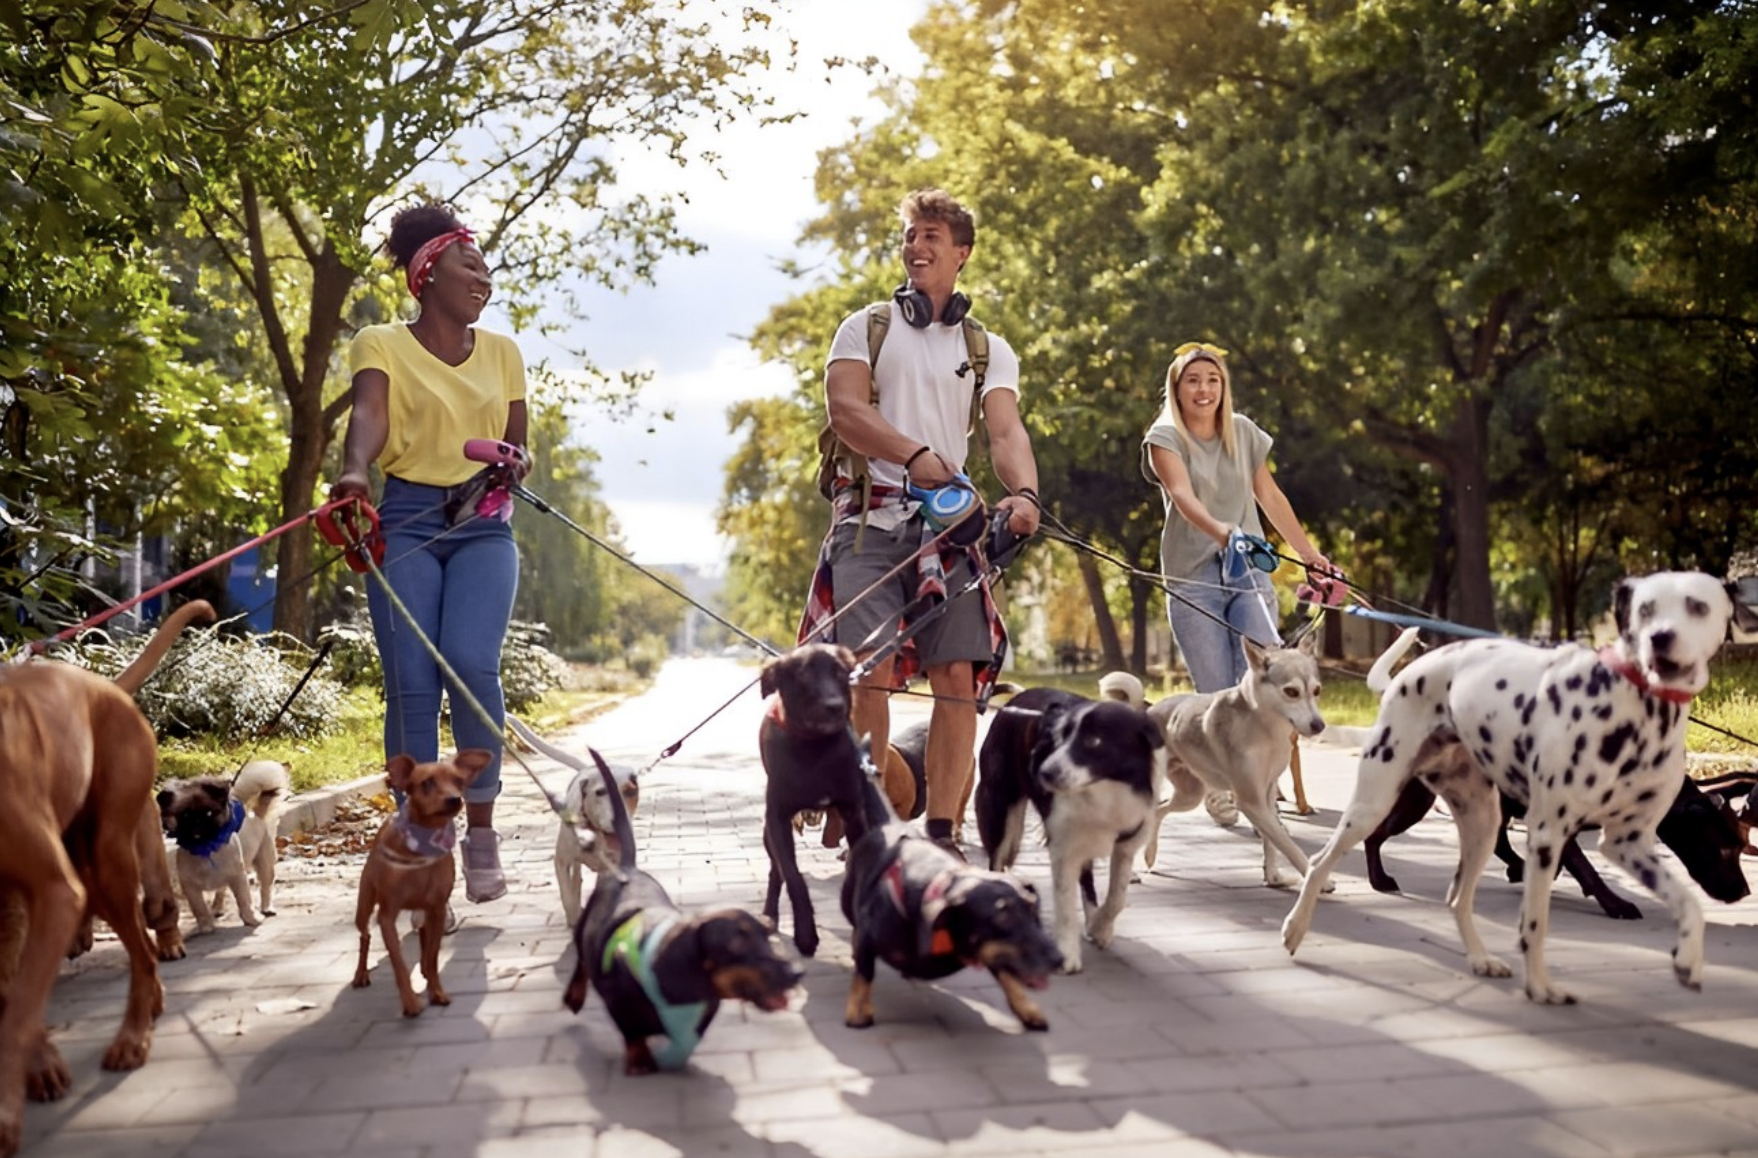
\includegraphics[width=0.7\linewidth]{imgs/img3.1.png}
    \caption{Una rappresentazione analogica di una situazione quotidiana}
\end{figure}

\begin{myobservation}[(Cosa c'è in una rappresentazione analogica)]
    Considera la rappresentazione analogica illustrata nell'immagine della Figura 3.1. Possiamo vedere tre persone, che possiamo assumere abbiano i nomi Paolo, Stefania e Sofia, che sono amici, vari cani, il fatto che siano uno a destra dell'altro e, naturalmente, molto altro.    
\end{myobservation}

\begin{myintuition}[(Fatto)]
    Un fatto \verb+f+ è un qualcosa che succede certamente ad una certa coordinata spaziotemporale
\end{myintuition}

\begin{mydefinition}[(Modello)]
    Un modello \verb+M+ è un set di fatti \verb+F = {f}+
    \begin{equation}
        \verb+M = {f}+
    \end{equation}
\end{mydefinition}

\begin{myobservation}[(Fatti e modelli)] I fatti sono gli elementi atomici, non ulteriormente decomponibili, di un modello. Nota che, a differenza dei modelli, i fatti sono considerati come una nozione primitiva e quindi non possono essere definiti formalmente.
\end{myobservation}

\begin{myexample}[(I fatti di un modello rappresentato nella Figura 3.1)]
    Un modello, uno tra molti altri, della situazione rappresentata nella Figura 3.1 potrebbe contenere, ad esempio, i seguenti fatti:
    \begin{verbatim}
    Sofia è una persona         Paolo è un uomo
    Rocky è un cane             Sofia è vicina a Paolo
    Sofia ha i capelli biondi   Sofia è un'amica di Paolo
    Rocky è un animale          Rocky è il cane di Sofia
    \end{verbatim}
\end{myexample}

\begin{myobservation}[(La soggettività dei fatti)]
    I fatti sono ciò che viene osservato e anche descritto, ad esempio, a terze persone. Il problema è che, proprio a causa di quanto discusso nella Sezione 2.2 e, nello specifico, il fatto di cosa siano i fatti è soggettivo e nascosto nelle menti delle persone che li percepiscono. Quanti altri fatti più e/o diversi da quelli elencati nell'Esempio 3.2 potresti immaginare? Potrebbero essere infiniti! Nota che ogni fatto può essere decomposto in qualsiasi insieme di fatti più semplici se questo è l'attuale focus dell'osservatore. Quindi, per esempio, anziché concentrarsi su Sofia, potrei concentrarmi sui suoi capelli, sulle sue gambe o su...
\end{myobservation}

\begin{myobservation}[(Fatti mutualmente (in)coerenti in un modello)]
    Il modello dell'Esempio 3.2 potrebbe essere esteso per affermare il fatto che Sofia è una donna o che Paolo è una persona. Tuttavia, avremmo problemi nell'estenderlo aggiungendo il fatto che Paolo è una donna o che Sofia è un cane, poiché avremmo due fatti mutualmente inconsistenti, qualcosa che sappiamo non può accadere nel mondo come lo percepiamo. Vedi anche l'Osservazione 2.9. Un modello non può contenere fatti che, almeno intuitivamente, sono mutualmente inconsistenti. Oltre a questo semplice esempio, la questione è come formalizzare questa intuizione e quindi come essere in grado di rilevarla mediante il ragionamento sui modelli.
\end{myobservation}

\begin{myobservation}[(Fatti e affermazioni)]
    Per essere considerato un fatto, deve essere descritto linguisticamente come tale. Non è per caso che nell'Esempio 3.2 abbiamo indicato i fatti attraverso un insieme di descrizioni in linguaggio naturale. Chiamiamo tali descrizioni "affermazioni". Il modo più semplice di pensare a un'affermazione è come a una frase dichiarativa in linguaggio naturale articolata in termini di un soggetto che si trova in una relazione più o meno complessa con un oggetto (come ad esempio, "Stefania sta camminando con i cani verso il centro della città"), o di un soggetto che detiene.
\end{myobservation}


\section{Teorie asserzionali}
\begin{myobservation}[(Affermazioni e teorie assertive)]
    Le affermazioni sono descrizioni indivisibili, diciamo atomiche, di un fatto. Le teorie assertive sono descrizioni di modelli.
\end{myobservation}

\begin{myintuition}[(Affermazione)]
    Un'affermazione $a$ è una rappresentazione linguistica atomica di un certo fatto \verb+f+.
\end{myintuition}

\begin{mydefinition}[(Teoria assertiva)]
    Una teoria assertiva $\mathcal{T}_A$ è un insieme di affermazioni.
    \begin{equation}
        \mathcal{T}_A = \{a\}
    \end{equation}

Abbiamo bisogno di definire che un'affermazione è la descrizione di un fatto specifico e, più in generale, che una teoria assertiva descrive un modello.

\begin{myexample}[(Una teoria assertiva del modello rappresentato nella Figura 3.1)]
    Una teoria assertiva, una tra molte altre, che descrive i fatti dell'Esempio 3.2 in linguaggio naturale potrebbe essere, ad esempio:
    \begin{verbatim}
    Sofia è una persona         Paolo è un uomo
    Sofia è vicina a Paolo      Rocky è il cane di Sofia
    Sofia è un’amica di Paolo   Sofia ha i capelli biondi
    Rocky è un cane             Rocky è un animale
    \end{verbatim}

\end{myexample}

Come si può notare, la teoria assertiva è in italiano, poiché essendo in linguaggio naturale può essere espressa anche in questo modo, e potrebbe essere altrettanto espressa in inglese.

\end{mydefinition}

\section{Funzioni d'interpretazione}
\begin{mydefinition}[(Funzione d'interpretazione)]
    Sia $\mathcal{I}_A$ una funzione di interpretazione di una teoria assertiva, definita come:
    \begin{equation}
        \mathcal{I}_A : \mathcal{T}_A \rightarrow \verb|M|
    \end{equation}
    Diciamo che un fatto \verb+f+ $\in$ \verb+M+ è l'interpretazione di $a \in \mathcal{I}_A$, e scriviamo:
    \begin{equation}
        \verb|f| = \mathcal{I}_A(a) = a^{\mathcal{I_A}}
    \end{equation}
    per intendere che $a$ è una descrizione linguistica di \verb|f|. Diciamo che \verb|f| è l'interpretazione di $a$, o, equivalentemente, che a denota \verb|f|.
(Più asserzioni possono portare ad un fatto)
\end{mydefinition}

\begin{myobservation}[(Funzione di interpretazione, polisemia)]
    Si assume che $\mathcal{I}_A$ sia una funzione, ovvero per ogni fatto esiste solo un'affermazione che lo descrive. In effetti, dobbiamo garantire che se due fatti $f_1$ e $f_2$ 
    sono diversi, allora non possono entrambi essere il risultato dell'interpretazione della stessa affermazione $a$, ovvero non può essere che se $\mathcal{T}_A = f_1$ allora anche $\mathcal{T}_A = f_2$. 
    Questo fenomeno, chiamato polisemia, è diffuso nelle lingue naturali ed è una delle principali fonti di malintesi e, di conseguenza, di costruzione di rappresentazioni mentali divergenti della stessa rappresentazione. 
    La polisemia delle affermazioni deriva direttamente dalla polisemia delle parole. Ad esempio: il nome proprio Java ha tre significati, è un linguaggio di programmazione, un tipo di chicchi di caffè e un'isola. La parola "auto" ha vari significati, ad esempio può significare automobile o una parte di un treno. 
    Parole generali, come "fare", hanno più di dieci significati. La polisemia è comune alla maggior parte delle parole, in particolare con quelle parole che vengono più comunemente utilizzate (le persone tendono a dare alle parole il proprio significato specifico) ed è una delle principali complicazioni (se non l'unica) che sorgono durante la costruzione di sistemi di comprensione del linguaggio naturale.
\end{myobservation}

\begin{myobservation}[(La non ambiguità delle funzioni di interpretazione)]
    Come dalla Sezione 1.3, le descrizioni linguistiche sono ambigue. Come dall'Osservazione 3.7, una delle principali ragioni è la polisemia delle parole. Tuttavia, questa ambiguità è nella mente dell'ascoltatore/lettore. Si può assumere che chi parla/scrive abbia sempre in mente l'analoga rappresentazione unica che sta descrivendo. La nozione di funzione di interpretazione impone questa supposizione, obbligando chi parla/scrive a essere esplicito sul significato inteso.
\end{myobservation}

\begin{myobservation}[(Funzione di interpretazione, sinonimia)]
    Due affermazioni sono sinonimi quando hanno lo stesso significato, ovvero l'interpretazione di due affermazioni diverse 
    $a_1$ e $a:$ può denotare lo stesso fatto $f$, ovvero $\mathcal{I}_A(a_1) = I_A(a_2) = f$. Le parole sinonime sono nuovamente diffuse nelle lingue naturali, in particolare con le entità più comuni. Le persone e le entità in generale hanno più nomi, ad esempio nome, cognome, nome più cognome, soprannomi, che sono sinonimi. Diverse lingue generano diversi nomi per la stessa entità (ad esempio, Gran Bretagna, Great Britain). Ci sono anche sostantivi sinonimi, ad esempio auto e automobile. Nota come la parola "auto" sia sia polisemica che sinonima. Anche questo è abbastanza comune. In generale, la sinonimia non è un problema. Tuttavia, nei database relazionali, la sinonimia non è consentita, essenzialmente per motivi di efficienza. I database sono sviluppati sulla base dell'assunzione del nome unico, ovvero nei database, stringhe e affermazioni diverse significano sempre cose diverse.
\end{myobservation}

\begin{myexample}[(Una funzione di interpretazione che fornisce un'interpretazione della teoria assertiva che descrive la Figura 3.1)]
    La funzione di interpretazione naturale che interpreta le frasi nell'Esempio 3.3 (sinistra) nei fatti dell'Esempio 3.2 (destra) è la seguente:
    \begin{FlushLeft}
        \hspace{1cm}
        \parbox{\dimexpr\linewidth-1cm}{
            $\mathcal{I}_A$(Sofia è una persona) = Sofia is a person \linebreak
            $\mathcal{I}_A$(Paolo è un uomo) = Paolo è un uomo \linebreak
            $\mathcal{I}_A$(Rocky è un cane) = Rocky è un cane \linebreak
            ...
            }

    \end{FlushLeft}
\end{myexample}

\begin{myobservation}[(Affermazioni e fatti, soggettività)]
    Il problema della soggettività delle rappresentazioni rimane, essendo un fatto inevitabile della vita. Tuttavia, le nozioni di fatto, affermazione e funzione di interpretazione forniscono uno strumento. In primo luogo, si assume che i fatti siano descritti in modo inequivocabile, tramite funzioni di interpretazione, dalle affermazioni che, a loro volta, sono rappresentazioni linguistiche e, come tali, possono essere condivise. In secondo luogo, le affermazioni, anche se selezionate soggettivamente dagli esseri umani, si presume siano atomiche, cioè forniscono il livello minimo possibile di dettagli con cui un modello può essere descritto.    
\end{myobservation}
\clearpage
\begin{figure}[ht]
    \centering
    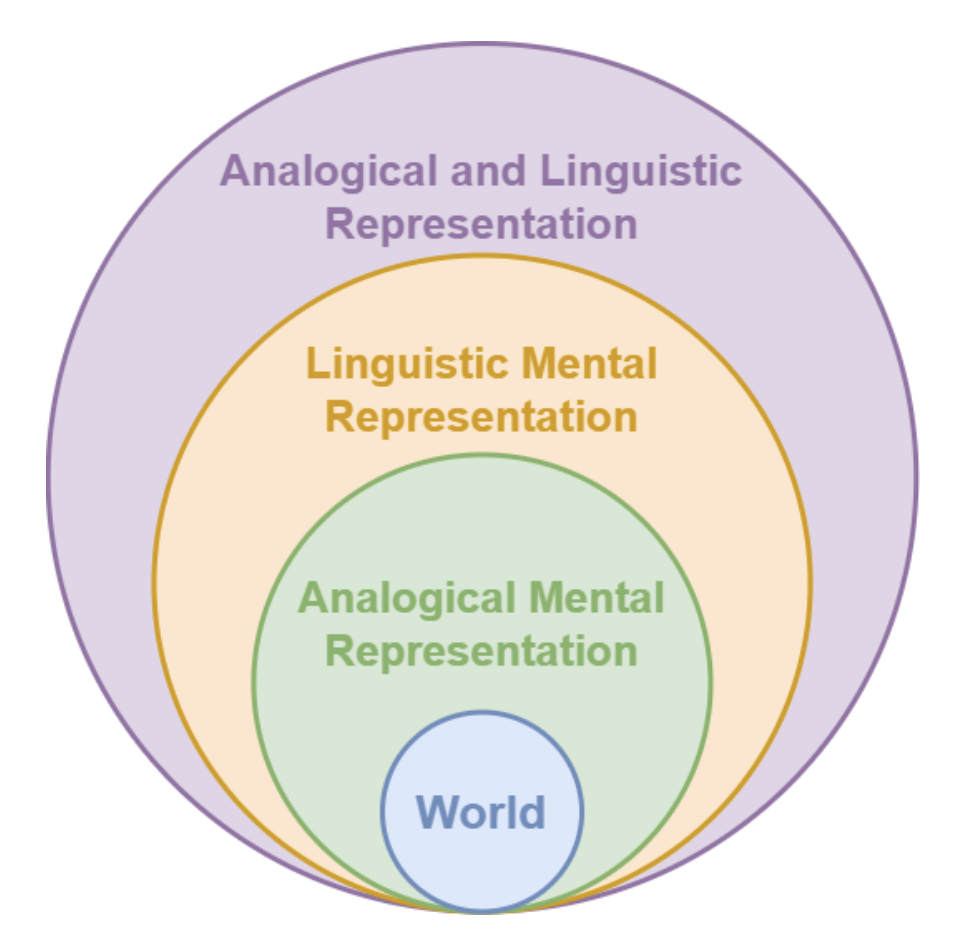
\includegraphics[width=0.7\linewidth]{imgs/img3.2.png}
    \caption{Diagramma di rappresentazione}
\end{figure}

\chapter{Modelli formali e teorie asserzionali}
Per evitare un ragionamento fallace, è necessario rappresentare modelli e teorie assertive in modo inequivocabile, ovvero formale. Quattro sono le caratteristiche che ci interessano:
\begin{itemize}
    \item \textbf{Formalità}: dovrebbe essere un linguaggio logico, ovvero con una sintassi e una semantica ben definite;
    \item \textbf{Universalità}: dovrebbe essere in grado di rappresentare tutti i tipi di fatti;
    \item \textbf{Intuitività}: dovrebbe consentire affermazioni i cui elementi di base (nomi di entità, concetti e proprietà) così come la loro struttura (ovvero come gli elementi di base sono collegati per costruire affermazioni) dovrebbero essere, da un lato, intuitivi per le persone mentre, dall'altro lato, avere una mappatura diretta alla struttura e all'organizzazione del dominio di riferimento;
    \item \textbf{Efficienza} computazionale: $\mathcal{L}_A$ dovrebbe consentire un motore di inferenza veloce ed efficiente, sfruttando l'efficienza intrinseca delle strutture dati utilizzate per memorizzare il modello del mondo.
\end{itemize}

\begin{myobservation}[(Tipi di linguaggi assertivi)]
    I modelli ER e UML sono intuitivi ma non universali, rappresentano solo fatti di conoscenza. I database sono computazionalmente efficienti ma rappresentano solo fatti di dati. Il linguaggio naturale è universale ma la sua semantica non è formalmente definita e non è computazionalmente efficiente. Quest'ultima debolezza si estende anche a sottoinsiemi ben definiti delle lingue naturali. Come esempio di questo caso, i linguaggi logici sono universali con sintassi e semantica ben definite, ma non sono intuitivi da comprendere e anche computazionalmente inefficienti (vedi anche la Sezione 6.5).    
\end{myobservation}

Nella Sezione 4.1, introduciamo alcune definizioni di base della teoria degli insiemi, utili per definire D, mentre, nella Sezione 4.2, introduciamo alcune definizioni di base della teoria dei grafi utili per definire $\mathcal{L}_A$.


    
\section{Teoria degli insiemi}
\subsection{Definizioni base}
Possiamo definire gli insiemi in due modi:
\begin{itemize}
    \item \textbf{Per elencazione}: L'insieme è descritto elencando tutti i suoi elementi (ad esempio, $A=\{a,e,i,o,u\}$).
    \item \textbf{Per astrazione}: L'insieme è descritto attraverso una proprietà dei suoi elementi (ad esempio, $A=\{x|x \text{è una vocale dell'alfabeto latino}\}$).
\end{itemize}

Abbiamo le seguenti definizioni di base.

\begin{mydefinition}[(Insieme vuoto)]
    $\emptyset$ è l'insieme che non contiene alcun elemento.
\end{mydefinition}

\begin{mydefinition}[(Appartenenza)]
    $a \in A$, l'elemento $a$ appartiene all'insieme $A$.
\end{mydefinition}

\begin{mydefinition}[(Non appartenenza)]
    $a \notin A$, l'elemento $a$ non appartiene all'insieme $A$.
\end{mydefinition}

\begin{mydefinition}[(Uguaglianza)]
    $A = B$, se e solo se $A$ e $B$ contengono gli stessi elementi.
\end{mydefinition}

\begin{mydefinition}[(Disuguaglianza)]
    $A \neq B$, se e solo se non è vero che $A = B$.
\end{mydefinition}

\begin{mydefinition}[(Sottoinsieme)]
    $A \subseteq B$, se e solo se tutti gli elementi in $A$ appartengono anche a $B$.
\end{mydefinition}

\begin{mydefinition}[(Sottoinsieme proprio)]
    $A \subset B$, se e solo $ \subseteq B$ e $A \neq B$.
\end{mydefinition}

\begin{mydefinition}[(Insieme universale)]
    L'insieme universale è l'insieme di tutti gli elementi o membri di tutti gli insiemi correlati e è denotato dalla lettera $\mathcal{U}$
\end{mydefinition}

Utilizziamo i \textbf{diagrammi di Venn} per rappresentare gli insiemi. I diagrammi di Venn consistono in cerchi sovrapposti o intersecati che rappresentano insiemi e le loro relazioni. Ogni cerchio rappresenta un insieme specifico, e l'area in cui i cerchi si sovrappongono rappresenta gli elementi condivisi tra gli insiemi corrispondenti. Un elemento che non appartiene a un insieme è rappresentato come un punto al di fuori del cerchio che rappresenta l'insieme.

\begin{mydefinition}[(Unione)]
    Dati due insiemi $A$ e $B$, l'unione di $A$ e $B$ è definita come l'insieme che contiene gli elementi appartenenti a $A$ o a $B$ o ad entrambi, e viene denotata con $\mathbf{A \cup B}$
\end{mydefinition}

\begin{figure}[ht]
    \centering
    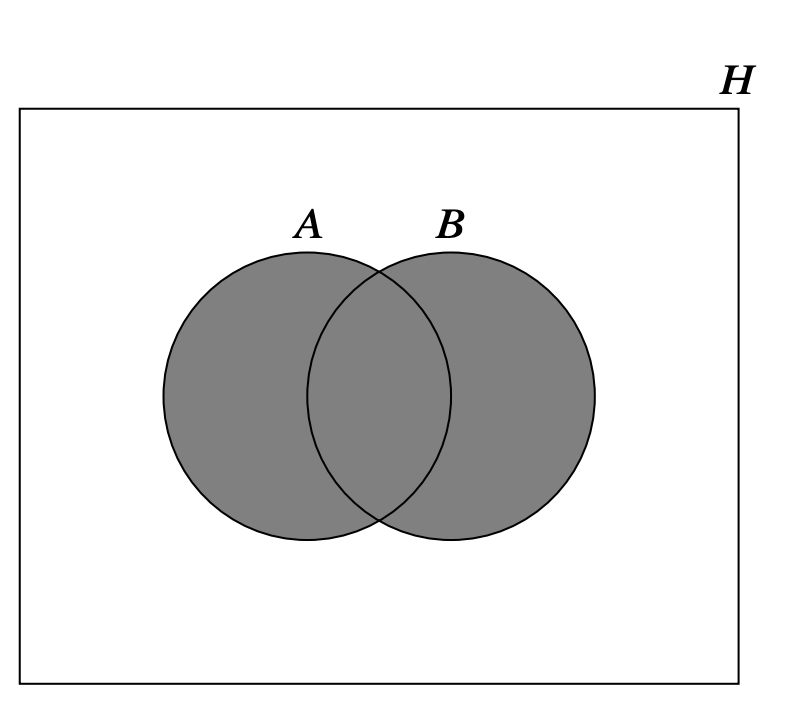
\includegraphics[width=0.3\linewidth]{imgs/img4.1.png}
    \caption{Operazione di unione}
\end{figure}


\begin{mydefinition}[(Intersezione)]
    Dati due insiemi $A$ e $B$, l'intersezione di $A$ e $B$ è definita come l'insieme che contiene gli elementi appartenenti sia a $A$ sia a $B$, e viene denotata con $\mathbf{A \cap B}$
\end{mydefinition}

\begin{figure}[ht]
    \centering
    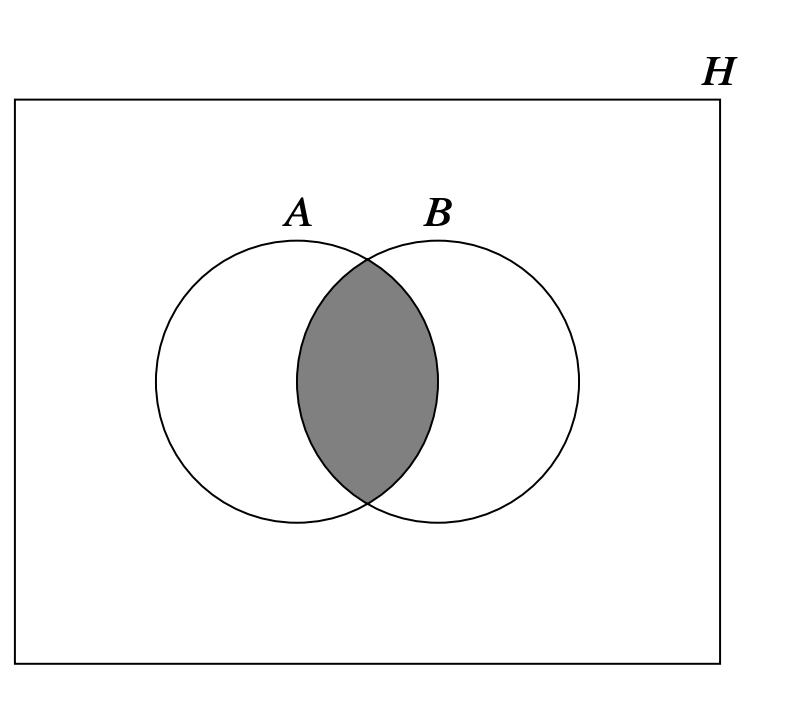
\includegraphics[width=0.3\linewidth]{imgs/img4.2.png}
    \caption{Operazione di intersezione}
\end{figure}


\begin{mydefinition}[(Differenza)]
    La differenza tra due insiemi $A$ e $B$, è definita come l'insieme che contiene gli elementi che sono membri di $A$, ma non membri di $B$. Viene denotata con $\mathbf{A \setminus B}$
\end{mydefinition}

\begin{figure}[ht]
    \centering
    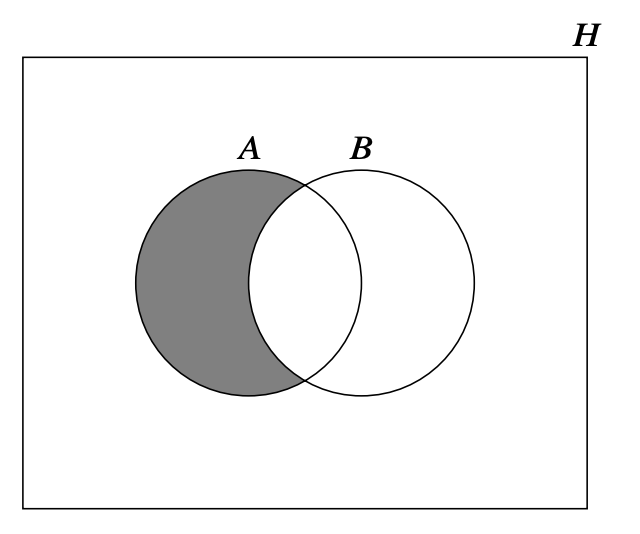
\includegraphics[width=0.3\linewidth]{imgs/img4.3.png}
    \caption{Operazione di differenza}
\end{figure}


\begin{mydefinition}[(Differenza complementare)]
    Dato un insieme universale $U$ e un insieme $A$, dove $A \subseteq U$, il complemento di $A$ in $U$  è definito come l'insieme che contiene tutti gli elementi in $U$ che non appartengono ad $A$ e viene denotato con $\mathbf{A^c}$ o $\mathbf{U \setminus A}$
\end{mydefinition}

\begin{figure}[ht]
    \centering
    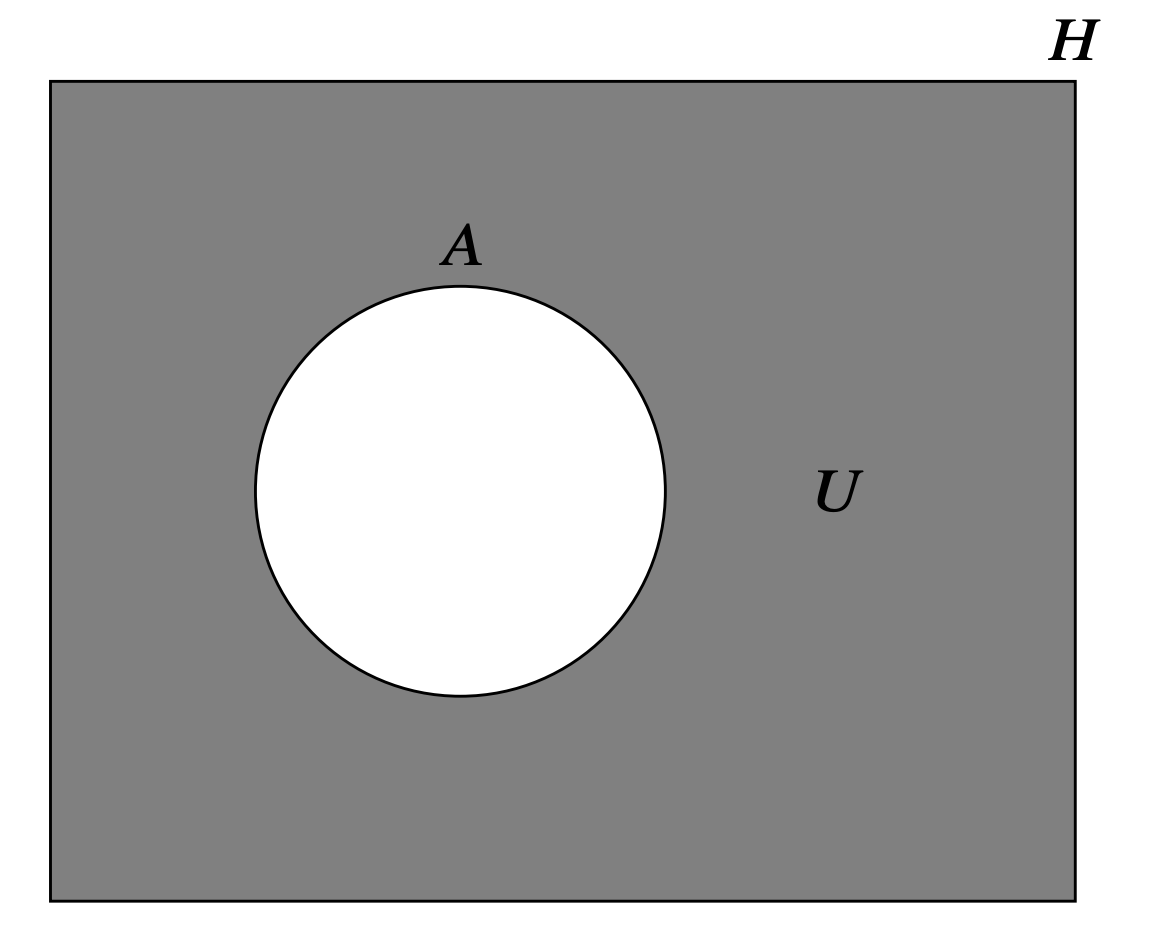
\includegraphics[width=0.3\linewidth]{imgs/img4.4.png}
    \caption{Differenza complementare}
\end{figure}

\begin{mytheorem}[(Proprietà delle operazioni)]
    \begin{outline}
        \1 \textbf{Con lo stesso set}
            \2 $A \cap A = A$
            \2 $A \cup A = A$

        \1 \textbf{Commutativa}
            \2 $A \cap B = B \cap A$
            \2 $A \cup B = B \cup A$

        \1 \textbf{Insieme vuoto}
            \2 $A \cap \emptyset = \emptyset$
            \2 $A \cup \emptyset = A$

        \1 \textbf{Associative}
            \2 $(A \cap B) \cap C = A \cap (B \cap C)$
            \2 $A \cap (B \cup C) = (A \cup B) \cap (A \cup C)$

        \1 \textbf{Leggi di De Morgan}
            \2 $\overline{A \cup B} = \overline{A} \cap \overline{B}$
            \2 $\overline{A \cap B} = \overline{A} \cup \overline{B}$

    \end{outline}
\end{mytheorem}

    \subsection{Relazioni}
    \subsection{Funzioni}
\section{Teorie dei grafi}
    \subsection{Nozioni base}
    \subsection{Grafi ...}
\section{Esercizi}

\chapter{Modello del Mondo - Rappresentazione Estensionale}
Le teorie assertive e i modelli rappresentano un passo importante avanti, ma ci sono ancora tre limitazioni principali:
\begin{itemize}
    \item Stiamo considerando solo i fatti del modello in esame. Cosa succede con i fatti che possono verificarsi negli altri possibili modelli, descrivendo situazioni possibilmente molto diverse?
    \item Il linguaggio utilizzato è molto limitato e consiste solo nell'insieme di affermazioni che descrivono i fatti del modello in esame. Cosa succede alle affermazioni che descrivono fatti in tutti gli altri modelli?
    \item Come conseguenza dei due fatti sopra, la definizione di funzione di interpretazione non è generale. Una nuova e diversa funzione di interpretazione deve essere definita per ogni nuova situazione.
\end{itemize}

\section{Dominio}
Secondo l'Equazione (3.1), un modello \verb|M| è deifinito come \verb|M = {f}|, dove \verb|f| è un insieme di fatti che sono veri in una determinata situazione.
\begin{mydefinition}[Dominio (di interpretazione)]
    Un dominio (di interpretazione) è un insieme di fatti \verb|{f}|
    \begin{equation}
        \verb|D| = \verb|{F}|
    \end{equation}
\end{mydefinition}

\begin{mydefinition}[(Modello)]
    Dato un dominio \verb|D|, un modello \verb|M| è un sott'insieme di \verb|D|
    \begin{equation}
        \verb|M| = \verb|{f}| \subseteq D
    \end{equation}
\end{mydefinition}

\begin{myobservation}[(Dominio, modello)]
    Un dominio è l'insieme di tutti i fatti che siamo disposti a considerare. Un modello è semplicemente il sottoinsieme di fatti che definiamo come rappresentativi di ciò che è il caso nella situazione attuale. La Definizione 5.2 generalizza in modo ovvio la Definizione 3.1.    
\end{myobservation}

\begin{myexample}[(I fatti del dominio rappresentato in Figura 3.1)]
    Un dominio che raccoglie, tra gli altri, i fatti rappresentati nella Figura 3.1 potrebbe contenere, ad esempio, i seguenti fatti:
    \begin{verbatim}
    Sofia is a person       Sofia is a woman
    Paolo is a man          Paolo is a person
    Paolo is a dog          Rocky is a dog
    Sofia is near Paolo     Rocky is the dog of Sofia
    Rocky is the dog of Paolo . . .
    \end{verbatim}
    ... e molti altri
\end{myexample}

\begin{myobservation}[(Dominio)]
    Mentre un modello è l'insieme di fatti che sono veri in una certa situazione, un dominio consiste nell'insieme di fatti che potenzialmente possono essere veri per tutte le possibili situazioni. Un dominio definisce tutto e solo ciò che può essere potenzialmente percepito.
\end{myobservation}

\begin{myobservation}[(Fatti mutuamente inconsistenti in un dominio)]
    Come dall'Esempio 5.1, un dominio, a differenza di un modello, può contenere fatti che, almeno intuitivamente, sono mutuamente inconsistenti. Dato un dominio, ci sono molti modelli potenziali, alcuni dei quali potenzialmente mutuamente inconsistenti. I domini devono consentire la possibile istanziazione di modelli distinti mutuamente inconsistenti, come avviene normalmente nel mondo.
\end{myobservation}


\section{Linguaggio asserzionale}
Secondo l'Equazione (3.2), una teoria assertiva $\mathcal{T}_A$ è definita come $\mathcal{T}_A=\{a\}$, dove $\{a\}$ è un insieme di affermazioni che descrivono i fatti che sono veri in una determinata situazione.

\begin{mydefinition}[(Linguaggio assertivo)]
    Un linguaggio assertivo $mathcal{L}_A$è un insieme di affermazioni $\{a\}$
    \begin{equation}
        \mathcal{L}_A = \{a\}
    \end{equation}
\end{mydefinition}

\begin{mydefinition}[(Teoria asserzionale)]
    Data un linguaggio assertivo $\mathcal{L}_A$, una teoria assertvia $\mathcal{T}_A$ è un sottonsieme di $\mathcal{L}_A$
    \begin{equation}
        \mathcal{T}_A = \{a\} \subseteq \mathcal{L}_A
    \end{equation}
\end{mydefinition}

\begin{myobservation}[(Linguaggio assertivo)]
    Mentre una teoria assertiva è l'insieme di affermazioni che descrive ciò che è vero in un certo modello, un linguaggio assertivo consiste nell'insieme di affermazioni che descrivono tutti i fatti che possono potenzialmente verificarsi. La Definizione 5.4 si estende in modo ovvio dalla Definizione (3.2).
\end{myobservation}

\begin{myexample}[(Linguaggio assertivo)]
    Il linguaggio dell'Esempio 3.3 esteso per includere tutti i fatti del dominio definito nell'Esempio 5.1 allo stesso modo (ossia, traduzioni italiane citate della frase in inglese che descrive un fatto) è un linguaggio assertivo.
\end{myexample}

\begin{myobservation}[(Completezza e correttezza di un linguaggio assertivo $\mathcal{L}_A$ rispetto a un dominio $D$)]
    Un linguaggio assertivo non è necessariamente completo, ovvero non contiene necessariamente affermazioni per tutti i fatti in un dominio (che, tra le altre cose, sono in principio infiniti). La caratteristica chiave è che dovrebbe contenere tutte le affermazioni ritenute rilevanti. Viceversa, un linguaggio assertivo è richiesto di essere corretto, cioè di contenere solo affermazioni che denotano fatti nel dominio di riferimento, al fine di evitare affermazioni prive di senso.
\end{myobservation}

\begin{myexample}[(Linguaggi assertivi):]
    \begin{enumerate}
        \item Linguaggi che consentono solo affermazioni in linguaggio naturale della forma "$<$soggetto$>$ $<$verbo$>$ $<$oggetto$>$" descrivono fatti sul mondo. Il linguaggio utilizzato è una sequenza di affermazioni semplici senza frasi complesse.
        \item I database relazionali (DB) descrivono fatti sul mondo. Il linguaggio utilizzato per descrivere i contenuti di un database relazionale sono le tabelle;
        \item I modelli entity-relationship (ER) descrivono fatti generali sui contenuti dei database. Sono scritti utilizzando il linguaggio del diagramma ER, un linguaggio di grafi specificamente etichettato.
        \end{enumerate}
\end{myexample}

\section{Funzione d'interpretazione}
\begin{mydefinition}[(Funzione di interpretazione)]
    Sia $\mathcal{L}_A$ un linguaggio di asserzioni e \verb|D| un dominio. Quindi, una Funzione di Interpretazione di un linguaggio assertivo $\mathcal{I}_A$ è definita come:

    \begin{equation}
        \mathcal{I}_A : \mathcal{L}_A \rightarrow \verb|D| \quad (\mathcal{I}_A \subseteq \mathcal{L}_A \times \verb|D|)
    \end{equation}

\end{mydefinition}

Vedi 3.3 (ripetizione) ... Andiamo avanti

\section{Modello del mondo}
Il viaggio è completo. Dobbiamo soltanto mettere tutto insieme.

\begin{myobservation}[(I ruoli di D,\(\mathcal{L}, \mathcal{I}_A, M, \mathcal{T}_A\))]
    Le definizioni fornite nelle sezioni precedenti possono essere riassunte dalla seguente figura.
    \begin{equation}
        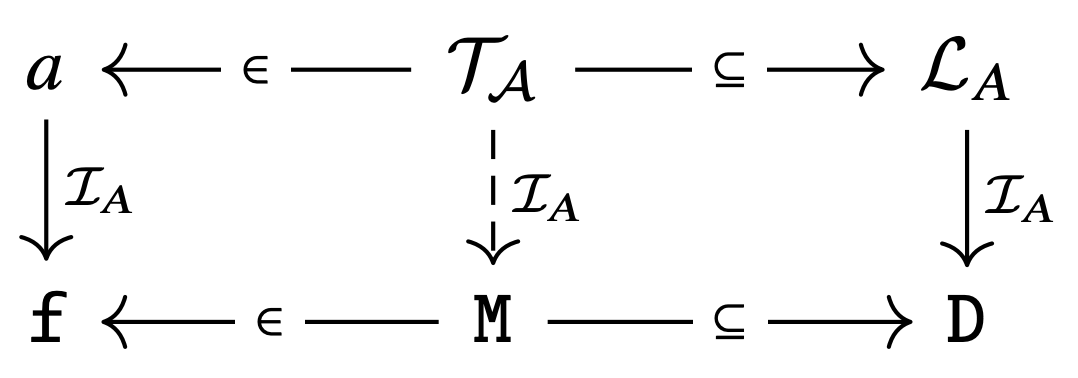
\includegraphics[height=15ex]{imgs/eq5.6.png}
    \end{equation}

\end{myobservation}

Nell'Equazione (5.7), \verb|D| definisce l'insieme di fatti $f$ di potenziale interesse, \verb|M| l'insieme di fatti su cui ci stiamo concentrando, $\mathcal{L}_A$  l'insieme di affermazioni $a$ di potenziale interesse e, infine, $\mathcal{T}_A$ è la teoria che descrive \verb|M|. In altre parole, come singole affermazioni $a$ descrivono singoli fatti f da un lato, e come gli insiemi complessivi di affermazioni $\mathcal{L}_A$ descrivono \verb|D| dall'altro lato, definiscono l'ambito entro il quale una teoria assertiva $\mathcal{T}_A$ può concentrarsi per descrivere modelli specifici \verb|M|. Affermazioni, linguaggi e teorie sono semplicemente i mezzi per specificare il modello desiderato enunciando i fatti desiderati tra quelli consentiti dal dominio di riferimento.
\begin{mydefinition}[(Modello del mondo)]
    \begin{equation}
        \hat{\mathcal{W}} = \langle \mathcal{L}_A, \verb|D|, \mathcal{I}_A \rangle 
    \end{equation}
    è un \textbf{modello del mondo}
\end{mydefinition}

\begin{myobservation}[(Modello del mondo)]
    Nell'Equazione (5.7), i componenti di un modello del mondo, cioè $\mathcal{L}_A, \verb|D|, \mathcal{I}_A$ definiscono le regole generali che vengono seguite durante la costruzione di una rappresentazione. Sono definiti a priori, di solito da esperti di modellizzazione e rappresentazione della conoscenza, come strumenti generali da utilizzare da parte degli operatori. Forniscono l'infrastruttura generale di modellazione che consente di rappresentare problemi del mondo reale. Forniscono anche un quadro uniforme con il quale è possibile confrontare e, eventualmente, anche unire due rappresentazioni. Gli sviluppatori di software di solito studiano questi modelli durante alcuni corsi di informatica o intelligenza artificiale e li utilizzano così come sono nello sviluppo di sistemi; si pensi, ad esempio, all'ampio utilizzo dei modelli ER (Entity-Relationship).
\end{myobservation}

\begin{myobservation}[(Dalle rappresentazioni mentali ai modelli del mondo)]
    I modelli del mondo sono spazi di rappresentazioni possibili, cioè teorie, progettati per minimizzare la possibilità di diverse rappresentazioni mentali della stessa teoria e del corrispondente modello che raffigura il mondo.
\end{myobservation}

I modelli del mondo forniscono il quadro generale entro il quale le teorie assertive e i modelli possono essere definiti e confrontati.

\begin{myobservation}[(Teoria e modello)]
    Ricorda che, dato un modello di un mondo $\hat{\mathcal{W}} = \langle \mathcal{L}_A, \verb|D|, \mathcal{I}_A \rangle$, abbiamo che $\verb|M| = \verb|{F}| \subseteq \verb|D|$ (equazione 5.1) e $\mathcal{T}_A = \{a\} \subseteq \mathcal{L}_A$ (equzione 5.3)
\end{myobservation}

\begin{myobservation}[(Definire un modello attraverso una teoria)]
    Il modo più comune per modellare il mondo è definire un insieme di affermazioni, ciò che chiamiamo una teoria. In altre parole, costruiamo un modello \verb|M| selezionando qualsiasi sottoinsieme $\mathcal{T}_A$ di $\mathcal{L}_A$. Questo è l'approccio comune quando il compito è rappresentare da zero una parte data del mondo che è di interesse.
\end{myobservation}

Tuttavia, a volte, viene fornita una teoria predefinita $\mathcal{T}_A$ e un modello predefinito \verb|M| e si chiede come sono correlati. In tal caso, abbiamo quanto segue.

\begin{mydefinition}[Correttezza e completezza di una teoria assertiva \(\mathcal{T}_A\) rispetto a un modello M]
    Sia $\hat{\mathcal{W}} = \langle \mathcal{L}_A, \verb|D|, \mathcal{I}_A \rangle$ il modello di un mondo. Siano $\mathcal{T}_A \subseteq \mathcal{L}_A$ e \verb|M| $\subseteq$ \verb|D| rispettivamente una teoria assertiva e un modello. Allora abbiamo due situazioni possibili, come segue:
    \begin{itemize}
        \item \textbf{Correttezza}. Sia $a$ $\in$ $\mathcal{L}_A$ un'asserzione. Se per tutte le $a$, se $a \in \mathcal{T}_A$ allora $\mathcal{I}_A(a) = \verb|f| \in \verb|M|$ diciamo che $\mathcal{T}_A$ è corretta rispetto a \verb|M|, o che \verb|M| è un modello per \textit{AL}.
        \item \textbf{Completezza}. Sia $\verb|f| \in \verb|M|$ un fatto. Se, per ogni \verb|f|, se $\verb|f| \in \verb|M|$ allora esiste un'asserzione $a \in \mathcal{T}_A$ tale che $\mathcal{I}_A(a) = \verb|f|$ diciamo che $\mathcal{T}_A$ è completa rispetto a \verb|M|.
      \end{itemize}

    Le nozioni di \textbf{scorrettezza} e \textbf{incompletezza} sono definite in modo ovvio.
\end{mydefinition}

\begin{myobservation}[(Correttezza e completezza di una teoria assertiva \(\mathcal{T}_A\) rispetto a un modello M)]
    Una teoria assertiva potrebbe non essere completa, ovvero potrebbero esistere fatti nel dominio per i quali non contiene affermazioni. Descrizioni incomplete dei modelli sono la norma, a causa dell'ignoranza o anche per mancanza di interesse. Tuttavia, una teoria $\mathcal{T}_A$ deve contenere solo affermazioni riguardanti i fatti in \verb|M| per \verb|M| appartenente a $\mathcal{T}_A$. Questo al fine di evitare informazioni errate. Notare come questo requisito sia opposto a quello su linguaggi e domini come indicato nell'Osservazione 5.5.
\end{myobservation}

\begin{myexample}[(Correttezza e completezza di una teoria assertiva \(\mathcal{T}_A\) rispetto a un modello M)]
    Considera l'Esempio 3.4. Una teoria assertiva $\mathcal{T}_A$ che contiene tutte e solo le affermazioni del dominio della funzione di interpretazione nell'Esempio 3.4 è corretta e completa rispetto al modello \verb|M| che contiene tutti e solo i fatti che sono nel dominio della stessa funzione di interpretazione. Qualsiasi teoria assertiva che è un sottoinsieme di $\mathcal{T}_A$ è corretta rispetto a \verb|M|. \verb|M| non è un modello di alcun superset di $\mathcal{T}_A$.
\end{myexample}


\chapter{Modello del Mondo - Rappresentazione Intenzionale}

I modelli del mondo ci permettono di sfruttare fatti e affermazioni su di essi come i principali componenti necessari per costruire una rappresentazione del mondo, da utilizzare successivamente per risolvere problemi.

\begin{myobservation}[(Modello del mondo, rappresentazione estensionale)]
    I modelli del mondo, come dalla Definizione 5.6, sono rappresentazioni estensionali del mondo, ovvero sono definite come insiemi di affermazioni $a$ e fatti $\verb|f|$, oltre a una funzione di interpretazione $\mathcal{I}_A$ che consente di definire quali affermazioni denotano quali fatti in uno o più modelli di riferimento.
\end{myobservation}

Ma cosa si intende per "fatto"? Come costruiamo affermazioni sui fatti? La risposta a questa domanda richiede la definizione di una rappresentazione intenzionale dei modelli del mondo, ovvero i meccanismi di rappresentazione che consentono di costruire affermazioni e fatti a partire da un insieme finito di elementi componenti primitivi. In seguito, ogni volta che è necessario per evitare confusione, adottiamo la seguente notazione e terminologia.

\begin{mynotation}[(Rappresentazione estensionale e intenzionale di un insieme)]
    Sia $\mathcal{S}$ un insieme. Allora con:
    \begin{itemize}
        \item $\mathcal{S}^e$ intendiamo la rappresentazione estensionale di $\mathcal{S}$, ovvero come un insieme di elementi (ad esempio, fatti, affermazioni, ma non solo);
        \item $\mathcal{S}^i$ intendiamo la rappresentazione intenzionale di $\mathcal{S}$, in cui gli elementi di $\mathcal{S}^e$ sono definiti intenzionalmente, a partire da un insieme di componenti primitivi. 
    \end{itemize}
    Gli apici vengono omessi quando non sorgono confusioni.
\end{mynotation}
    
\section{Dominio}
L'Esempio 3.1, l'Osservazione 3.1 e anche l'Osservazione 3.5 forniscono indicazioni su come costruire una rappresentazione intenzionale dei fatti.

\begin{myintuition}[(Dominio, rappresentazione intenzionale)]
    La rappresentazione intenzionale di un dominio è composta da tre componenti, come segue:
    \begin{itemize}
        \item \textit{entità}, associate agli elementi della rappresentazione che possono essere isolati e distinti dal resto;
        \item \textit{classi} (insiemi) di entità, caratterizzate dal fatto di avere alcune caratteristiche comuni non condivise dalle entità degli altri insiemi;
        \item \textit{relazioni} tra entità, che raccolgono più entità che condividono una proprietà comune.
    \end{itemize}
\end{myintuition}

\begin{mydefinition}[(Dominio, rappresentazione intenzionale)]
    La rappresentazione intenzionale $\verb|D|^i$ di un dominio $\verb|D|$ è definita come:

    \begin{equation}
        \verb|D|^i = \langle E, \{C\}, \{R\} \rangle 
    \end{equation}

    con

    \begin{gather}
        \nonumber E = \{e\}\\
        \nonumber C \subseteq E\\
        \nonumber R \subseteq E \times \dots \times E \textnormal{ n times}
    \end{gather}

    dove $E = \{e\}$ è un set di \textbf{identità}, $\{C\}$ è un set di \textbf{classi} di identità, $\{R\}$ p un insieme di relazione $n$-arie $R^n$ per qualche $n$. $E$ viene chiamato l'universo di $D^i$ o anche \textbf{l'universo dell'interpretazione}.

\end{mydefinition}

\begin{mydefinition}[(Fatto, rappresentazione intensionale)]
    La rappresentazione intensionale di un fatto \(\verb|f|\) assume una delle quattro seguenti forme.
    \begin{equation}
        \begin{aligned}
            \mathrlap{\texttt{e}} \hphantom{\langle \texttt{e}_1, \dots, \texttt{e}_n \rangle} &\in \verb|C| \\
            \mathrlap{\langle \texttt{e}_1, \dots, \texttt{e}_n \rangle} \hphantom{\langle \texttt{e}_1, \dots, \texttt{e}_n \rangle} &\in \verb|R| \\
            \mathrlap{\texttt{C}} \hphantom{\langle \texttt{e}_1, \dots, \texttt{e}_n \rangle} &\subseteq \verb|E| \\
            \mathrlap{\texttt{R}^n} \hphantom{\langle \texttt{e}_1, \dots, \texttt{e}_n \rangle} &\subseteq \verb|C|_1 \times \dots \times \verb|C|_n
         \end{aligned}
    \end{equation}
    con $\verb|e, e|_i \in \verb |E|$ e $\verb|C, C|_i \subseteq \verb|E|$.
\end{mydefinition}

\begin{myobservation}[(Fatto, rappresentazione intensionale)]
    L'intuizione dietro la Definizione 6.2 è la seguente. $e \in C$ significa che una certa entità $e$ appartiene a una certa classe $C$, come nel caso dell'affermazione che Sofia è una persona. $<e_1, \ldots, e_n> \in R$ significa che $n$ entità si trovano in una certa relazione, come nel caso dell'affermazione che Paolo si trova tra Sofia e Stefania. $C \subseteq E$ significa che $C$, ad esempio "persona", è una classe. $R_n \subseteq C_1 \times \ldots \times C_n$ significa che una relazione si applica solo a classi specifiche, come nel caso dell'affermazione che le persone sono amiche degli animali.
\end{myobservation}

\begin{myobservation}[(Complessità dei fatti)]
    Si potrebbe pensare a fatti più sofisticati, ad esempio il fatto $C_1 \subseteq C_2$. Ciò è naturalmente possibile, a costo di complicare il linguaggio assertivo, con un limite superiore nell'intuitività del modello di mondo risultante. Qui stiamo definendo il modello di mondo più semplice possibile. Tuttavia, i linguaggi di rappresentazione e le logiche possono comunque essere utilizzati per aumentare l'espressività del linguaggio di rappresentazione.
\end{myobservation}

\begin{myexample}[(Fatto, rappresentazione intensionale ed estensionale)]
    Consideriamo l'Esempio 5.1. Il fatto che Sofia sia una persona è costruito prendendo l'entità Sofia e affermando che essa è una persona. Il fatto che Sofia sia vicina a Paolo è costruito affermando che le entità Sofia e Paolo stanno in una relazione in cui una è vicina all'altra.
\end{myexample}

\begin{mydefinition}[(Dominio, rappresentazione estensionale)]
    La rappresentazione estensionale $D_e$ di un dominio $D$, la cui rappresentazione intensionale $D_i$ è come da Definizione 6.1, è $D_e = \{f\}$ con $f$ come da Definizione 6.2.
\end{mydefinition}

\begin{myobservation}[(Entità)]
    Ma cosa si intende per entità? L'idea generale è che un'entità è qualcosa che può essere percepito e quindi rappresentato in una rappresentazione analogica di (una parte del) mondo. È un'entità un oggetto specifico? O una persona? O un animale? Sì, ma anche qualsiasi cosa che avvenga nel tempo, ad esempio un evento o un processo. Si assume che le entità abbiano nomi. Esempi di (nomi di) entità: Federico, Pussy, Garfield, Trento, l'ultimo Campionato del Mondo di calcio, e così via.
\end{myobservation}

\begin{myintuition}[(Entità)]
    Un'entità è qualsiasi cosa che può essere rappresentata in una rappresentazione (analogica o linguistica) del mondo e che ha un nome. Un'entità può essere rappresentata nella rappresentazione mentale del mondo ogni volta che è percepita o il suo nome è udito da un essere umano.
\end{myintuition}

\begin{myintuition}[(Nome)]
    Un nome è una stringa, scritta in qualche lingua, che consente di fare riferimento alle entità nelle rappresentazioni e, più specificamente, nei modelli di mondo.
\end{myintuition}

\begin{myintuition}[(Entità nominata)] 
    Il vigneto di fronte a me non è un'entità (per me). Anche se posso vederlo chiaramente, non ho un nome che posso usare per fare riferimento ad esso, ad esempio quando parlo con gli altri. Per essere considerate entità, devono essere entità nominate.
\end{myintuition}

\begin{myobservation}[(Dominio, rappresentazione intensionale)] 
    Modelliamo intenzionalmente il mondo intorno a noi in termini di entità. Le entità, a loro volta, sono raggruppate in classi specifiche, in base a determinate loro proprietà. Quindi abbiamo, ad esempio, le classi: umano, persona, donna, animale, cane, macchina, penna, computer, e così via. Le entità possono essere messe in relazione tra loro in base alla loro classe. Ad esempio: gli esseri umani sono amici degli esseri umani, o degli animali, mangiano cibo, una macchina è vicina a un semaforo e così via.
\end{myobservation}

\begin{myobservation}[(Dominio, parzialità)]
     Un dominio non deve contenere tutti e cinque i tipi di fatti elencati nella Definizione 6.2. La selezione dei fatti da includere dipende da ciò che si sta modellando. Grossolanamente, i domini possono essere suddivisi in due tipi. Il primo è il dominio dei dati, così chiamato perché descrive ciò che è percepibile e coinvolge i primi due tipi di fatti nella Definizione 6.2. Il secondo tipo è il dominio della conoscenza, così chiamato perché si concentra su affermazioni generali, non direttamente percebili, e descrive relazioni generali tra classi e relazioni. I domini della conoscenza coinvolgono gli ultimi tre tipi di affermazioni. Esistono anche quelli che qui chiamiamo domini misti, ovvero domini che coinvolgono tutti i tipi di fatti. I domini misti sono molto utili nella comunicazione, ad esempio nella comunicazione in linguaggio naturale tra le persone, poiché consentono di esprimere uniformemente la conoscenza sulle entità, le classi e le relazioni.
\end{myobservation}

\begin{mydefinition}[(Dominio, dati, conoscenza, misto)]
    Un dominio dei dati contiene solo fatti della forma $e \in C$ e $<e_1, \ldots, e_n> \in R$. Un dominio della conoscenza contiene solo fatti della forma $C_1 \subseteq E$ e $R_n \subseteq C_1 \times \ldots \times C_n$. Un dominio misto contiene tutti i tipi di fatti.
\end{mydefinition}

\begin{myexample}[(Dominio dei dati)]
    Il dominio descritto nell'Esempio 5.1 è un dominio dei dati. Alcuni dei suoi fatti possono essere rappresentati intenzionalmente come segue:
\begin{align*}
\text{sofia} &\in \text{Person} \\
<\text{rocky}, \text{paolo}> &\in \text{DogOf} \\
\text{sofia} &\in \text{Woman} \\
\text{paolo} &\in \text{Dog} \\
<\text{paolo}, \text{rocky}> &\in \text{HasDog} \\
\text{rocky} &\in \text{Dog} \\
<\text{sofia}, \text{paolo}> &\in \text{Near} \\
<\text{rocky}, \text{sofia}> &\in \text{DogOf} \\
\text{paolo} &\in \text{Man} \\
<\text{sofia}, \text{paolo}> &\in \text{FriendOf} \\
<\text{paolo}, \text{sofia}, \text{stefania}> &\in \text{Between}
\end{align*}
Nella notazione, le entità sono scritte con le lettere iniziali in minuscolo, mentre nei concetti e nelle proprietà sono in maiuscolo.
\end{myexample}

\begin{myexample}[(Dominio della conoscenza)] Un dominio della conoscenza che descrive la conoscenza alla base del dominio dei dati nell'Esempio 5.1 è un dominio dei dati che potrebbe contenere, ad esempio, i seguenti fatti:
\begin{align*}
\text{Person} &\subseteq \text{Entity} \\
\text{HasDog} &\subseteq \text{Person} \times \text{Dog} \\
\text{Dog} &\subseteq \text{Entity} \\
\text{DogOf} &\subseteq \text{Dog} \times \text{Person} \\
\text{Animal} &\subseteq \text{Entity} \\
\text{FriendOf2} &\subseteq \text{person} \times \text{person} \times \text{person} \\
\text{Near} &\subseteq \text{Entity} \times \text{Entity} \\
\text{FatherOf} &\subseteq \text{Person} \times \text{Person} \\
\text{ChildOf} &\subseteq \text{Person} \times \text{Person}
\end{align*}
Dove "Entity" sta per $E$.
\end{myexample}

\begin{myexample}[(Dominio misto)]
    Un esempio di dominio misto può essere creato unendo i domini dell'Esempio 6.2 e 6.3.
\end{myexample}


\section{Linguaggi assertivi}
\begin{mydefinition}[(Linguaggio assertivo, rappresentazione intensionale)]
    La rappresentazione intensionale $L_{iA}$ di un linguaggio assertivo $L_A$ è definita come
    \begin{equation}
        L_{A}^i = \langle E, \{C\}, \{P\} \rangle
    \end{equation}
    dove $E = \{e\}$ è un insieme di (nomi di) entità, $\{C\}$ è un insieme di concetti, dove un concetto è un nome di una classe, e $\{P\}$ è un insieme di proprietà, dove una proprietà è un nome di una relazione.
\end{mydefinition}
    
\begin{mydefinition}[(Linguaggio assertivo, rappresentazione estensionale)]
    La rappresentazione estensionale $L_{A}^e$ di un linguaggio assertivo $L_A$, la cui rappresentazione intensionale $L_{A}^i$ è come da Definizione 6.5, è $L_{A}^e = \{a\}$ con $a$ che ha una delle seguenti quattro forme.
    \begin{equation}
        \begin{aligned}
            & C(e)\\
            & \mathcal{P}_n(e_1, \dots, e_n)\\
            & C\\
            & \mathcal{P}_n(C_1, \dots, C_n)
        \end{aligned}
    \end{equation}
    Dove: $C(e)$ dovrebbe essere letto come l'entità di nome $e$ appartenente alla classe di nome $C$, e $P(e_1, \ldots, e_n)$ come le entità di nome $e_1, \ldots, e_n$ coinvolte nella relazione di nome $P$.
\end{mydefinition}

\begin{myobservation}[(Sintassi astratta e concreta)]
    Le affermazioni nella Definizione 6.6 devono essere lette come sintassi astratta, anziché sintassi concreta. Devono essere prese come segnaposti per molteplici modi di descrivere lo stesso fatto in diverse lingue assertive. Quindi, ad esempio, l'asserzione di sintassi astratta Person(Sofia) è la rappresentazione di sintassi astratta di molteplici rappresentazioni di sintassi concrete, come ad esempio Person(Sofia), Sofia è una persona, P(S), (Sofia)Person (notazione postfix) e, soprattutto, varie tipologie di notazioni grafiche (vedi sotto). Ciò che conferisce significato alle affermazioni è il loro significato inteso, come definito dalla funzione di interpretazione (vedi sotto). In concreto, la sintassi utilizzata nelle prime due affermazioni proviene dalla logica $\mathcal{LOE}$, mentre quella delle ultime tre proviene dalla logica $\mathcal{LOD}$.
\end{myobservation}

\begin{myterminology}[(Alfabeto)]
    La rappresentazione intenzionale, come definita nella Definizione 6.6, $\mathcal{L}^i_A$, di un linguaggio, in questo caso $\mathcal{L}_A$, definito estensionalmente, in questo caso $\mathcal{L}^e_A$, è anche chiamata l'alfabeto (di quel linguaggio).
\end{myterminology}

\begin{myobservation}[(Alfabeto)]
    Le affermazioni descrivono fatti. Il primo passo è associare a ciascun elemento del dominio un nome nell'alfabeto del linguaggio assertivo. Successivamente, le affermazioni vengono costruite compositamente seguendo come sono costruiti i fatti. Ciò crea una corrispondenza uno-a-uno tra i fatti e le affermazioni, che suggerisce immediatamente il fatto descritto da un'affermazione.
\end{myobservation}

\begin{myobservation}[(Linguaggio assertivo, parzialità)]
    L'Osservazione 6.6 si estende in modo ovvio ai linguaggi assertivi.
\end{myobservation}

\begin{mydefinition}[(Linguaggio assertivo, dati, conoscenza, misto)]
    Un linguaggio assertivo di dati contiene solo affermazioni della forma $C(e)$ e $P(e1, \ldots, en)$. Un linguaggio assertivo di conoscenza contiene solo fatti della forma $C$ e $P_n(C1, \ldots, Cn)$. Un linguaggio assertivo misto contiene entrambi i tipi di affermazioni.
\end{mydefinition}

\begin{myexample} (Un linguaggio assertivo di dati che descrive il dominio dei dati nell'Esempio 6.2)
    Alcune affermazioni sono le seguenti:
    \begin{align*}
        & \text{Person(sofia)} && \text{Woman(sofia)} && \text{Man(paolo)} \\
        & \text{Person(paolo)} && \text{Dog(paolo)} && \text{Dog(rocky)} \\
        & \text{Near(sofia, paolo)} && \text{DogOf(rocky, sofia)} && \text{FriendOf(sofia, paolo)} \\
        & \text{DogOf(rocky, paolo)} && \text{HasDog(sofia, rocky)} && \text{HasFriend(paolo, sofia)}
    \end{align*}

\end{myexample}

\begin{myexample}[(Un linguaggio assertivo di conoscenza che descrive il dominio della conoscenza nell'Esempio 6.3)]
    Alcune affermazioni sono le seguenti:
    \begin{align*}
        & \text{Person} && \text{HasDog(Entity,Entity)} && \text{Woman} \\
        & \text{Dog} && \text{FriendOf2(Man,Man,man)} && \text{Animal} \\
        & \text{Near(Entity, Entity)} && \text{HasFriend(Man,Dog)} && \text{FriendOf1(Person, Person)}
    \end{align*} 
    dove "Entity" è il concetto che denota l'insieme Entity di tutte le entità nel dominio.
\end{myexample}

\begin{myexample}[(Un linguaggio assertivo misto che descrive il dominio misto negli Esempi 6.2, 6.3)]
    Alcune affermazioni sono le seguenti:
    \begin{align*}
        & \text{Person} && \text{Near(rocky, paolo)} && \text{Person(paolo)} \\
        & \text{FriendOf1(Person, Person)} && \text{FriendOf1(sofia, paolo)} && \text{Dog} \\
        & \text{Dog(rocky)} && \text{Near(Entity, Entity)} && \text{Near(paolo, sofia)}
    \end{align*}
    Le affermazioni di conoscenza implicano affermazioni sui dati. Pertanto, ad esempio, si potrebbe dedurre che Sofia è una persona dal fatto che è un amico di un'altra persona. Questo richiede ragionamento, cioè ciò per cui servono le logiche.
\end{myexample}

\begin{myexample}[(Un linguaggio assertivo di conoscenza, utilizzando modelli ER, che descrive il dominio della conoscenza nell'Esempio 6.3)]
    Consideriamo l'Esempio 6.6: concentriamoci sui seguenti concetti e ruoli:
    \begin{align*}
        & \text{Person} && \text{Animal} && \text{HasAnimal(Person, Animal)} \\
        & \text{OwnedBy(Animal, Person)} && \text{Woman} && \text{Man} \\
        & \text{Dog} && \text{HasDog(Man, Dog)} && \text{HasDog(Women, Dog)} \\
        & \text{OwnedBy(Dog, Man)} && \text{OwnedBy(Dog, Woman)}
    \end{align*}

    Here is a sample ER Model describing our example:
    \clearpage
    \begin{figure}[ht]
        \centering
        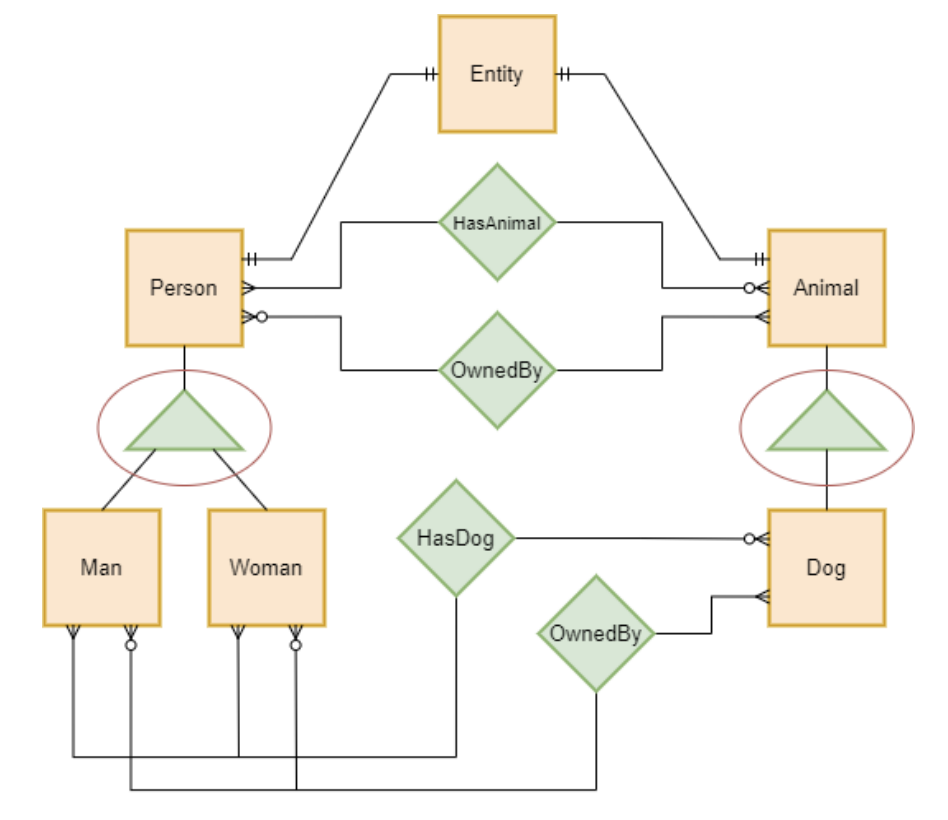
\includegraphics[width=0.7\linewidth]{imgs/img6.1.png}
        \caption{Modello ER}
    \end{figure}
\end{myexample}

Notazione: i quadrati rappresentano concetti, i rombi rappresentano relazioni, i triangoli
rappresentano una relazione IS-A (quindi, ad esempio, Uomo è un'istanza di Persona).
Si noti che i domini, come li abbiamo definiti, non consentono le relazioni IS-A (per il momento, vedere Osservazione 6.3). Ecco perché questa relazione non deve essere considerata per i linguaggi ER da considerarsi linguaggi assertivi. Per quanto riguarda le frecce, quella con due stanghe rappresenta una relazione uno a uno, mentre le frecce a forchetta rappresentano una relazione molti a molti, in cui quelle con un punto bianco identificano l'esistenza facoltativa della relazione.

\begin{myexample}[(Un linguaggio assertivo di dati, utilizzando database relazionali, che descrive il dominio dei dati nell'Esempio 6.2)]
    Considerando le affermazioni dell'esempio 6.1, ecco come i nostri dati sono rappresentati da un database:
    \clearpage
    \begin{figure}[ht]
        \centering
        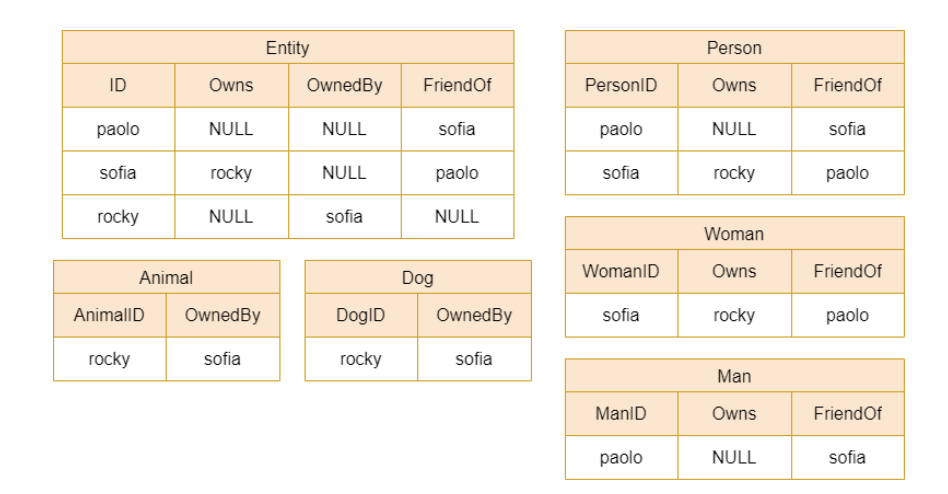
\includegraphics[width=0.7\linewidth]{imgs/img6.2.png}
        \caption{Database con dati}
    \end{figure}
    Notiamo come alcune caselle siano istanziate come NULL, questo avviene per mancanza di informazioni.
\end{myexample}

\begin{myexample}[(Un linguaggio assertivo di conoscenza, utilizzando schemi di database relazionali, che descrive il dominio della conoscenza nell'Esempio 6.2)]
    Invece, in questo esempio vediamo le relazioni delle diverse chiavi nel database (continuando a considerare le affermazioni nell'esempio 6.1):
    \begin{figure}[ht]
        \centering
        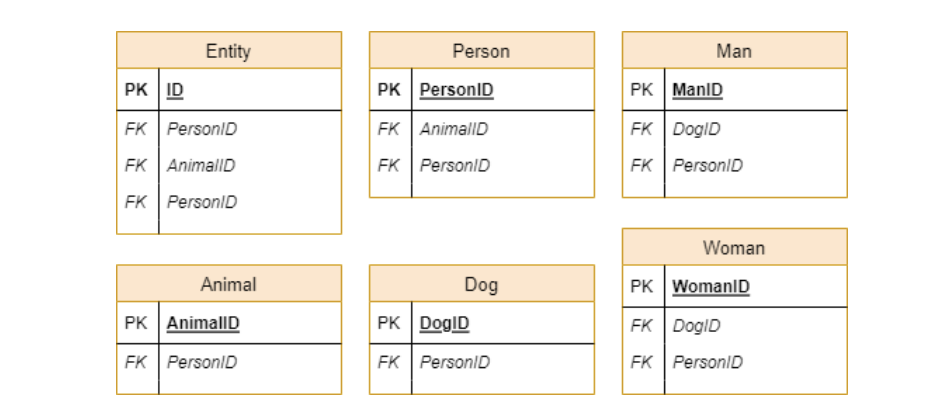
\includegraphics[width=0.7\linewidth]{imgs/img6.3.png}
        \caption{Relazione del Database}
    \end{figure}
    Notiamo come alcune caselle siano istanziate come NULL, questo avviene per mancanza di informazioni.
\end{myexample}

\begin{myobservation}[(Linguaggi assertivi, dati, conoscenza e misti)]
    I tre esempi chiariscono lo scopo e lo scopo dei linguaggi e dei domini di dati, conoscenza e misti. I linguaggi di dati, che descrivono fatti nel mondo reale, formalizzano il contenuto dei database (relazionali) o rappresentazioni analoghe (file CSV, JSON, XML). I linguaggi di conoscenza specificano la conoscenza di riferimento, ad esempio, relazioni, attributi, dei linguaggi di dati. I linguaggi misti vengono utilizzati per specificare entrambi.
\end{myobservation}



\section{Funzione d'interpretazione}
\begin{mydefinition}[(Funzione di interpretazione, interpretazione intensionale)]
    La rappresentazione intenzionale $I_i^A$ di una funzione di interpretazione $I_A : L_A \rightarrow D$ di un linguaggio assertivo è definita come segue:
    \begin{equation}
        \mathcal{I}^i_A = \langle \mathcal{I}_e, \mathcal{I}_C, \mathcal{I}_P \rangle
    \end{equation}
    con:
    \begin{equation}
        \begin{aligned}
            &\mathcal{I}_e : \mathcal{E} &&\rightarrow \verb|E| \\
            &\mathcal{I}_C : \{\mathcal{C}\} &&\rightarrow \verb|{E}| \\
            &\mathcal{I}_P : \{\mathcal{P}^n\} &&\rightarrow \verb|{E}| \times \dots \times \verb|{E}|
        \end{aligned}
    \end{equation}
    e di conseguenza:
    \begin{equation}
    \begin{aligned}
        I_\mathcal{A}(C(e)) &= I_\mathcal{C}(C)(I_\mathcal{E}(e)) &&= e \in C \\
        I_\mathcal{A}(P_n(e_1, \ldots, e_n)) &= I_{\mathcal{P}_n}(I_\mathcal{E}(e_1), \ldots, I_\mathcal{E}(e_n)) &&= \langle e_1, \ldots, e_n \rangle \in R_n \\
        I_\mathcal{A}(C) &= I_\mathcal{C}(C) &&= C \subseteq E \\
        I_\mathcal{A}(P_n(C_1, \ldots, C_n)) &= I_{\mathcal{P}_n}(I_\mathcal{C}(C_1), \ldots, I_\mathcal{C}(C_n)) &&= R_n \subseteq C_1 \times \cdots \times C_n
    \end{aligned}
\end{equation}
dove: $I_e$ è la funzione di interpretazione delle entità, $I_C$ è la funzione di interpretazione dei concetti e $I_P$ è la funzione di interpretazione delle proprietà.
\end{mydefinition}

\begin{mynotation}[(Notazione alternativa per la funzione di interpretazione)]
    L'equazione (6.7) è talvolta scritta come segue:
    \begin{equation}
        \begin{aligned}
            I_\mathcal{A}(C(e)) &= C^{I}(e^I) \\
            I_\mathcal{A}(P(e_i, e_j)) &= P^{I}(e^I_i, e^I_j) \\
            I_\mathcal{A}(C) &= C^{I} \\
            I_\mathcal{A}(P(C_i, C_j)) &= P^{I}(C^I_i, C^I_j)
        \end{aligned}
    \end{equation}
\end{mynotation}

\begin{myobservation} [(Funzione di interpretazione)]
    L'equazione (6.7) mostra come $I_A$ viene applicata ricorsivamente applicandola ai componenti della sua affermazione di input fino all'interpretazione delle entità. In questo processo, i suoi componenti vengono applicati come necessario, cioè $I_e$ alle entità, $I_C$ ai concetti e $I_P$ alle proprietà. La corrispondenza uno a uno tra il linguaggio e la struttura del dominio per costruire il significato di un'affermazione componendolo a partire dal significato dei suoi componenti.
\end{myobservation}

\begin{myobservation}[(Funzione di interpretazione, interpretazione intenzionale)]
    Quando $D_i$ e $L_i^A$ vengono costruiti seguendo le regole evidenziate nell'Osservazione 6.8 e $I_A$ è come nell'Equazione (6.7), allora la rappresentazione del mondo è intuitiva e autoesplicativa, mappata uno a uno con la rappresentazione analoga che sta descrivendo. Ciò consente allo sviluppatore della rappresentazione di concentrarsi solo sulle rappresentazioni linguistiche, pensando implicitamente alla corrispondente rappresentazione analogica.
\end{myobservation}

\begin{mydefinition}[(Funzione di interpretazione, dati, conoscenza, misto)]
    Una funzione di interpretazione dei dati mappa un linguaggio assertivo dei dati in un dominio dei dati. Una funzione di interpretazione della conoscenza mappa un linguaggio assertivo della conoscenza in un dominio della conoscenza. Una funzione di interpretazione mista mappa un linguaggio misto in un dominio misto.
\end{mydefinition}

\begin{myexample}[(Una funzione di interpretazione dei dati dal linguaggio dei dati nell'Esempio 6.5 al dominio dei dati nell'Esempio 6.2)]
    Un'istanza di applicazione è
    \begin{align*}
        I_A(FriendOf1(sofia, paolo)) = I_P(FriendOf1)(I_e(sofia), I_e(paolo))\\ = <sofia, paolo> \in FriendOf1
    \end{align*}
\end{myexample}

\begin{myexample}[(Una funzione di interpretazione della conoscenza dal linguaggio assertivo nell'Esempio 6.6 al dominio della conoscenza nell'Esempio 6.3)]
    Un'istanza di applicazione è
    \begin{align*}
        I_A(FriendOf1) = I_P(FriendOf1) = FriendOf1 \subseteq Person \times Person
    \end{align*}
\end{myexample}

\begin{myexample}[(Un'interpretazione della conoscenza dal linguaggio del modello ER nell'Esempio 6.1 al dominio della conoscenza nell'Esempio 6.3)]
    Un'istanza di applicazione è
    NECESSITA' DI IMMAGINE CON MAPPING DI UN CONCETTO E UN ELEMENTO DI PROPRIETÀ

\end{myexample}

\begin{myexample}[(Una funzione di interpretazione dei dati dal linguaggio del database nell'Esempio 6.9 al dominio dei dati nell'Esempio 6.2)]
    Un'istanza di applicazione è
    NECESSITA' DI IMMAGINE CON MAPPING DI UN ELEMENTO DI DATI COMMENTO SU COME MAPPARE NULL
\end{myexample}

\begin{myexample}[(Una funzione di interpretazione della conoscenza dal linguaggio dello schema del database nell'Esempio 6.15 al dominio della conoscenza nell'Esempio 6.2) ]
    Un'istanza di applicazione è
    NECESSITA' DI IMMAGINE CON MAPPING DI UN ELEMENTO DI DATI
\end{myexample}


\section{Modello del mondo}
\begin{mydefinition}[(Dominio del Mondo, rappresentazione intenzionale)]
    Dato un Dominio del Mondo \({\hat{W}}\) definito come
    \begin{equation*}
        {\hat{W}} = < L_A, D, I_A >
    \end{equation*}
        la sua rappresentazione intenzionale \({\hat{W^i}}\) è definita come
    \begin{equation}
        {\hat{W^i}} = < L_A^i, D_{i}, I_A^i >
    \end{equation}
    con
    \begin{align*}
        &L_A^i = < E, \{C\}, \{P\} >\\
        &D_i = < E, \{C\}, \{R\} >\\
        &I_A^i = < I_e, I_C, I_P >
    \end{align*}
    dove \(\hat{W^i}\) è (chiamato) il modello di mondo stencil, \(D_i\) è lo stencil del dominio, \(L^i_A\) è lo stencil del linguaggio (assertivo) e \(I^i_A\) è lo stencil della funzione di interpretazione.
\end{mydefinition}

\begin{myobservation}[(Lo stencil del modello del mondo)]
    \(\hat{W^i}\) è tutto ciò di cui abbiamo bisogno per definire un modello del mondo e per utilizzarlo per implementare teorie e modelli corrispondenti. Vedi le Osservazioni 5.13 e 5.14 e la Definizione 5.7.
\end{myobservation}

\begin{myterminology}[(Data, conoscenza, misto)]
    Parliamo di modelli di mondo, teorie e modelli di dati, conoscenza e misti con il significato ovvio.
\end{myterminology}

\begin{myobservation}[(Modello di mondo)]
    La Definizione 6.10 ci dice che un modello di mondo è composto da un linguaggio \(L_A\) di affermazioni su un dominio di riferimento \(D\), in cui il significato delle affermazioni in \(L_A\) è univoco nel senso che il fatto denotato da un'affermazione è definito in modo univoco dal ruolo chiave della funzione di interpretazione \(I_A\). In questo senso, vale la pena riassumere le proprietà chiave delle funzioni di interpretazione, come introdotte e discusse sopra.
    \begin{itemize}
        \item Non consente la polisemia: un elemento nel linguaggio denota uno e un solo elemento del dominio. L'ambiguità denotazionale non è possibile;
        \item Consente la sinonimia: un elemento del dominio può essere denotato da più di un elemento del linguaggio;
        \item È totale: ogni elemento del linguaggio ha una denotazione nel dominio di riferimento. Le affermazioni prive di significato non sono consentite;
        \item Non è (necessariamente) surgettivo: possono esistere elementi del dominio per i quali non esistono elementi nel linguaggio che li denotano.
        \item È compositivo: il significato di un'affermazione è calcolato mediante la composizione funzionale dei suoi elementi costitutivi. Il significato delle affermazioni è codificato intenzionalmente nella loro struttura.
    \end{itemize}
\end{myobservation}

\begin{myobservation}[(Definizione di un modello di mondo)]
    La costruzione di un modello di mondo \(\widehat{W} = < L_A, D, I_A >\) richiede di passare attraverso la definizione dei suoi tre componenti. La motivazione è di solito la necessità di modellare un determinato dominio di problema. Il modellatore di solito inizia con una comprensione intuitiva del dominio, anche se non è lavorata in dettaglio. Il processo di solito segue i seguenti passaggi:
    \begin{enumerate}
        \item Definire \(L_A\), dove l'idea chiave è che \(L_A\) dovrebbe catturare gli aspetti chiave del dominio di destinazione;
        \item Specificare \(D\) assicurandosi che sia una rappresentazione analogica adeguata del dominio di destinazione;
        \item Definire \(I_A\), in questo processo convalidando il fatto che \(L_A\) e \(D\) siano adeguatamente definiti e allineati reciprocamente.
    \end{enumerate}
    Spesso gli ultimi due passaggi, almeno inizialmente, vengono eseguiti solo in modo intuitivo, facendo affidamento sulla composizione della funzione di interpretazione. Questi passaggi di solito vengono eseguiti completamente solo quando il modello di mondo è stato utilizzato per un po' di tempo e le sue ambiguità, se presenti, sono diventate esplicite. Nel complesso, il processo di costruzione dei modelli di mondo è complesso, richiede molta esperienza. Potrebbe richiedere anni per definire completamente un modello di mondo.
\end{myobservation}

\begin{myexample}[(Definizione di un modello di mondo)]
    In tutta questa sezione, a partire dalla Sezione 2, abbiamo costruito modelli di mondo. Modelli di mondo semplici possono essere costruiti raccogliendo linguaggio, dominio e funzione di interpretazione da questi esempi e allineandoli in modo adeguato. Tuttavia, si noti che, come già menzionato in precedenza, la definizione dei modelli di mondo è un compito molto complesso che richiede molta competenza, validazione nel campo e, in ultima analisi, tempo. Come già menzionato in precedenza, i modelli ER, i modelli UML, sottoinsiemi del linguaggio naturale arricchiti con adeguate funzioni di interpretazione, sono esempi di modelli di mondo.
\end{myexample}

\begin{myobservation}[(Utilizzo di un modello di mondo - costruzione e ragionamento su una teoria del mondo)]
    Il problema è come descritto nella Sezione 1.3 e nella Sezione 2.2. Abbiamo un modello di mondo e dobbiamo utilizzare la sua struttura per costruire un insieme di affermazioni, cioè una teoria del mondo, e dobbiamo assicurarci di cosa essa rappresenta, ovvero il modello di riferimento, e le sue proprietà. Una volta che una teoria è articolata con riferimento a un modello di mondo, diventa possibile studiare le sue proprietà attraverso una metodologia generale e algoritmi definiti nella prossima sottosezione.
\end{myobservation}

L'aspetto chiave nella definizione o selezione di un modello di mondo è la decisione sul linguaggio assertivo \(L_A\) e il livello di ambiguità che esso permette.

\begin{myintuition}[(Linguaggio, informale, semi-formale, logico)]
    I linguaggi dei modelli di mondo sono di tre tipi, come segue:
    \begin{itemize}
        \item \textbf{Linguaggi informali}, ossia linguaggi in cui la sintassi di \(L_A\) è definita in modo informale, ad esempio, in linguaggio naturale e senza l'uso di regole di produzione.
        \item \textbf{Linguaggi semi-formali}, ossia linguaggi in cui la sintassi di \(L_A\) è definita formalmente.
        \item \textbf{Linguaggi formali}, chiamati anche linguaggi logici, ossia linguaggi in cui \(L_A\) e \(I_A\) sono definiti formalmente.
    \end{itemize}
\end{myintuition}

\begin{myexample}[(Linguaggio, informale, semi-formale, logico)]
    Con riferimento all'esempio precedente, abbiamo quanto segue:
    \begin{itemize}
        \item Linguaggi informali: tutte le lingue naturali;
        \item Linguaggi semi-formali: il linguaggio relazionale dei database, la notazione ER e UML;
        \item Linguaggi logici: i linguaggi utilizzati nella logica.
    \end{itemize}
\end{myexample}

\begin{myobservation}[(Linguaggio, informale, semi-formale, logico)]
    Abbiamo quanto segue.
    \begin{itemize}
        \item I linguaggi informali sono più facili da usare in quanto sono conosciuti da tutti. Nell'Informatica, vengono tipicamente utilizzati nella stesura dei requisiti iniziali, ad esempio, da mostrare ai clienti. La principale difficoltà è che c'è una elevata probabilità di fraintendimento. Ora vengono utilizzati anche nelle interazioni con i ChatBot.
        \item I linguaggi semi-formali vengono tipicamente utilizzati nell'Ingegneria del Software quando si scrivono requisiti avanzati. Riducono il livello di ambiguità e sono molto efficaci nel lavoro collaborativo tra gli Ingegneri del Software. Possono anche essere utilizzati nella generazione automatica di codice. Possono sorgere problemi a causa della presenza di un certo livello di ambiguità semantica.
        \item I linguaggi logici hanno due principali utilizzi: (i) La specifica di software e hardware altamente critici (ad esempio, sistemi critici per la sicurezza o la sicurezza) e (ii) l'implementazione di sistemi di ragionamento, tipicamente sistemi di Intelligenza Artificiale, in grado di calcolare le conseguenze da ciò che è noto.
    \end{itemize}
\end{myobservation}

\section{Utilizzare un modello di mondo}
Vediamo come i modelli di mondo possono essere utilizzati nella pratica per rappresentare e ragionare sul mondo. Ci concentriamo sui modelli di mondo logici.
\begin{figure}[ht]
    \centering
    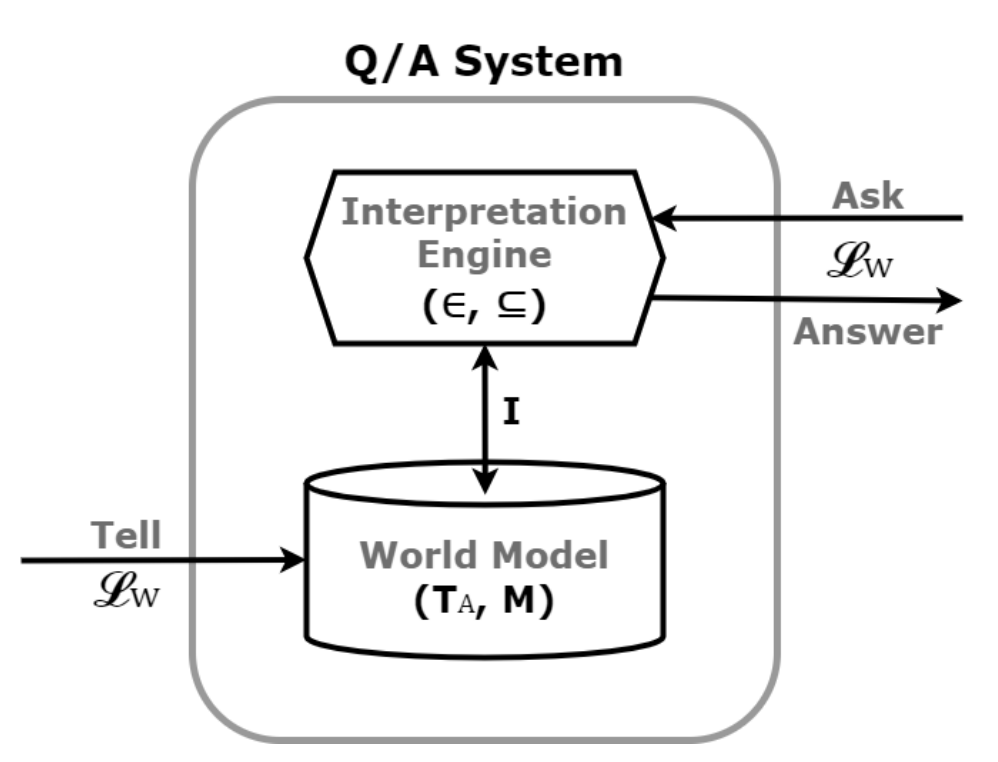
\includegraphics[width=0.7\linewidth]{imgs/img6.4.png}
    \caption{Risolvere problemi utilizzando il modello di mondo}
\end{figure}

\begin{myintuition}[(La risoluzione dei problemi mediante l'uso di modelli di mondo)]
    L'uso dei modelli di mondo può essere caratterizzato come una soluzione alla necessità di rispondere a domande (in linguaggio naturale) o query (in qualche linguaggio formale, ad esempio SQL) sul mondo, grazie allo sfruttamento di un meccanismo di ragionamento che consente di calcolare conseguenze da un corpo di conoscenza esistente sul mondo, cioè una teoria. Questo processo di solito si articola in tre compiti principali, come segue (vedi anche Figura 6.4):
    \begin{itemize}
        \item Comunicare Dati e Conoscenza, da un responsabile di sistema al sistema. Ciò richiede la specifica di un linguaggio \(L_T\) che può essere utilizzato per specificare i fatti del modello di mondo in uso.
        \item Porre una Domanda, da un utente al sistema, ovvero le domande / query specifiche su cui l'utente vuole conoscere le risposte. Ciò richiede la specifica di un linguaggio \(L_Q\) utilizzato per scrivere domande / query.
        \item Rispondere a una Domanda, dal sistema all'utente, riguardo alla domanda posta precedentemente, scritta in un linguaggio \(L_A\).
    \end{itemize}

Alcune osservazioni. Il responsabile e l'utente sono di solito persone diverse. Di solito il processo di fornire al sistema ulteriori informazioni è continuo nel tempo. Di solito \(L_Q\) e \(L_A\) sono lo stesso linguaggio \(L\). Molto spesso il linguaggio \(L_T\) è diverso sia da \(L_Q\) che da \(L_A\). Ci sono tre principali motivazioni per questo: efficienza del ragionamento, intuitività dell'interazione con l'utente e, non da ultimo, la necessità che \(L_T\) sia più adatto per la specifica del modello di mondo. Ad esempio, come sarà chiaro nel seguito, i modelli basati su grafi sono molto adatti per la specifica del modello di mondo, mentre \(L_Q\) e \(L_A\) sono spesso in (alcuni frammenti di) linguaggio naturale. La traduzione tra questi linguaggi è sempre automatica e implementata all'interno del sistema di domande e risposte.
\end{myintuition}

\begin{myterminology}[(Ne Il linguaggio del modello di mondo)]
    Nelle seguenti assumiamo che \(L_Q = L_A = L_T = L_W\), dove \(L_W\) è il linguaggio di rappresentazione del modello di mondo.
\end{myterminology}
\begin{mydefinition}[(Interpretazione e conseguenza)]
    Sia \(\hat{W} = <L_A, D, I_A>\) un modello di mondo. Sia \(T \subseteq L_A\) una teoria e \(M \in D\) un modello di \(\hat{W}\). Sia \(a \in T\) un'asserzione. Allora scriviamo
    \begin{equation}
        \begin{aligned}
            &M |= _{L_A} a \text{ to mean } I_A(a) \in M \\
            &M |= _{L_A} T \text{ to mean } I_A(a) \in M \text{ per ogni } a \in T
        \end{aligned}
    \end{equation}
    e diciamo che $M$ implica $T$, o anche che M implica \(a\). La notazione per il linguaggio \(L_A\) viene omessa quando non è necessaria.
\end{mydefinition}

\begin{myintuition}[(Modelli di mondo, problemi di ragionamento)]
    Ma quali domande e quali risposte? Tutti i modelli di mondo forniscono risposte a quattro (fondamentali) domande fondamentali che enunciamo di seguito come problemi di ragionamento. Supponiamo di avere un modello di mondo \(\hat{W}\) definito intensionalmente, cioè \(\hat{W^i} = <L_i, D_i, I_i>\) e che abbiamo un insieme {M} di modelli con \(M \subseteq D\) e un insieme di teorie \(T \subseteq L_A\). Allora abbiamo quanto segue (notare che un'asserzione si comporta come con un elemento):
\end{myintuition}

\begin{myreasoningproblem}[(Model checking)]
    Given T and M, check whether $M |= T$ .
\end{myreasoningproblem}

\begin{myobservation}[(Verifica del modello e correttezza della teoria)]
    La verifica del modello è la stessa cosa della verifica della correttezza di una teoria rispetto a un modello, come dalla Definizione 5.7. È sufficiente verificare se le asserzioni in T si verificano in M.
\end{myobservation}

\begin{myreasoningproblem}[(Satisfiability)]
    Given T , check whether there exists M such that $M |= T$ .
\end{myreasoningproblem}

\begin{myobservation}[(Soddisfacibilità)]
    Qualsiasi teoria che non rappresenti informazioni negative, come più spesso accade, è soddisfacibile. Se le informazioni negative sono consentite, è sufficiente verificare se la teoria contiene due fatti che si contraddicono reciprocamente.
\end{myobservation}

\begin{myobservation}[(Risposta alle query nei database)]
    La risposta alle query nei database è una forma sofisticata di verifica del modello / soddisfacibilità. Il contenuto del database è il modello di mondo di riferimento, la query è la teoria da verificare, la risposta è l'insieme di istanze che rendono corretta la teoria di input.
\end{myobservation}

\begin{myreasoningproblem}[(Validity)]
    Given T, check whether for all $M$, $M |= T$.
\end{myreasoningproblem}

\begin{myobservation}[(Validità)]
    Applicare la verifica del modello a tutti i modelli M.
\end{myobservation}

\begin{myreasoningproblem}[(Insoddisfacibilità)]
    Dato T, verificare se non esiste alcun M tale che $M |= T$.
\end{myreasoningproblem}

\begin{myobservation}[(Insoddisfacibilità)]
    Se le informazioni negative sono consentite, verificare due asserzioni contraddittorie.
\end{myobservation}

\begin{myintuition}[(Un'architettura per la risoluzione dei problemi mediante l'uso di modelli di mondo)]
    L'architettura che supporta l'uso dei modelli di mondo, come specificato nell'Intuizione 6.6, è rappresentata nella Figura 6.4. Possiamo identificare due componenti principali, come segue:
    \begin{itemize}
        \item Un motore di modelli di mondo (inferenza) che codifica i dati e le conoscenze disponibili sul mondo e consente un ragionamento minimo su di essi (vedere i problemi di ragionamento nell'Intuizione 6.7);
        \item Un motore di interpretazione (inferenza) che implementa uno o più dei problemi di ragionamento definiti nell'Intuizione 6.7.
    \end{itemize}
    Nota che il sistema viene selezionato all'inizio. La scelta dipende dalle specifiche del problema da risolvere.
\end{myintuition}

\begin{myobservation}[(Motore di inferenza del modello di mondo)]
    Il ragionamento in un modello di mondo equivale a verificare se una query (un'unica asserzione o un insieme di asserzioni come parte di una teoria) appartiene al modello. Query più sofisticate, come quelle implementate nei database relazionali, possono essere implementate in cui è possibile lasciare alcuni elementi della query non specificati. Il motore di inferenza troverà quindi il corretto s.
\end{myobservation}

\section{Esercizi}

\begin{myexercise}[(ER Creation)]
    Create an ER Model from this theory:
    \begin{itemize}
        \item There is a tree
        \item There is a banana
        \item The monkey is eating a banana
        \item The monkey is sitting on a tree*
        \item The monkey is scratching his head*
    \end{itemize}
\end{myexercise}

\begin{myexercise} \newline
    Considera le frasi e la modellazione della teoria. Dimmi se è completa, corretta, completa e corretta, incompleta o scorretta.

    \begin{minipage}{0.6\textwidth}
        \begin{itemize}
            \item A = "There is a banana"
            \item A = "There is a monkey"
            \item C = "There is a tree"
            \item D = "The monkey is eating a banana"        
        \end{itemize}    
    \end{minipage}%
    \begin{minipage}{0.4\textwidth}
        \centering
        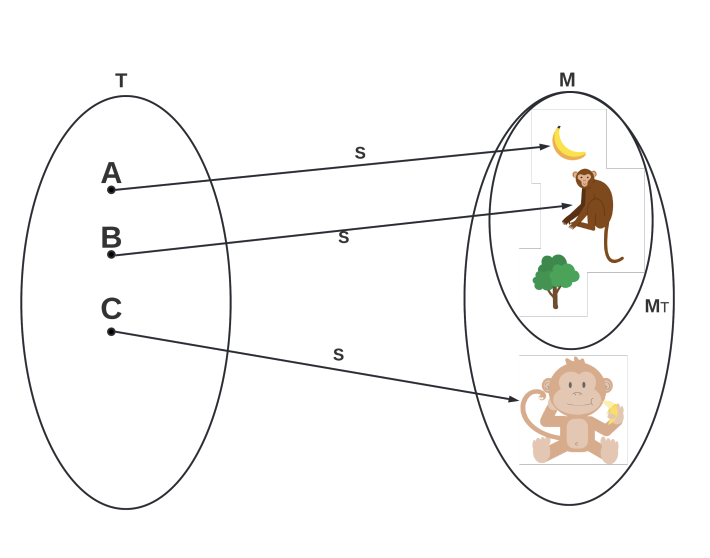
\includegraphics[width=\textwidth]{imgs/ex6.2.png}
    \end{minipage}
\end{myexercise}

\begin{myexercise} \newline
    Considera le frasi e la modellazione della teoria. Determina se è completa, corretta, completa e corretta, incompleta o errata.

    \begin{minipage}{0.6\textwidth}
        \begin{itemize}
            \item A = "There is a banana"
            \item A = "There is a monkey"
            \item C = "There is a tree"
            \item D = "The monkey is eating a banana"        
        \end{itemize}    
    \end{minipage}%
    \begin{minipage}{0.4\textwidth}
        \centering
        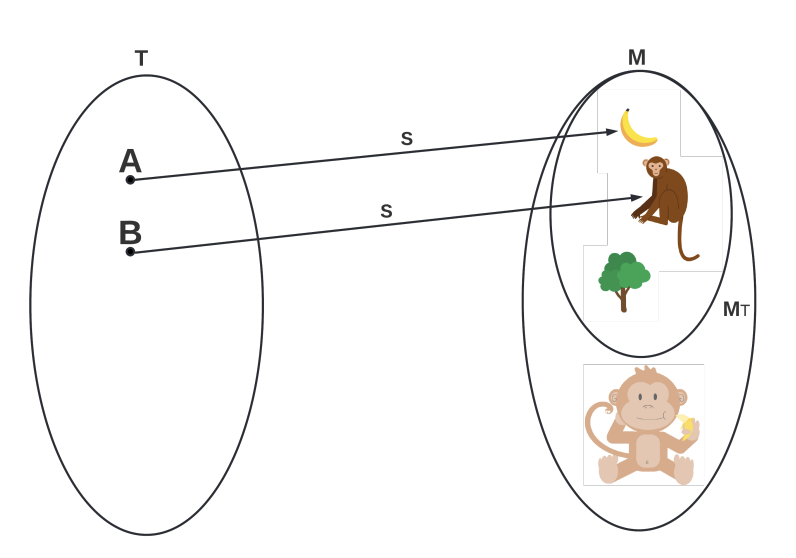
\includegraphics[width=\textwidth]{imgs/ex6.3.png}
    \end{minipage}
\end{myexercise}

\begin{myexercise} \newline
    Considera le frasi e la modellazione della teoria. Determina se è completa, corretta, completa e corretta, incompleta o errata.

    \begin{minipage}{0.6\textwidth}
        \begin{itemize}
            \item A = "There is a banana"
            \item A = "There is a monkey"
            \item C = "The monkey is eating a banana"
            \item D = "There is a tree"        
        \end{itemize}    
    \end{minipage}%
    \begin{minipage}{0.4\textwidth}
        \centering
        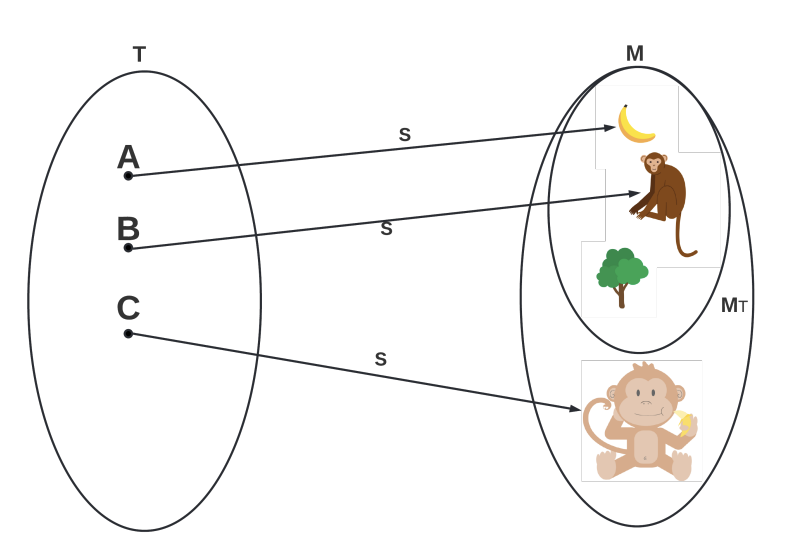
\includegraphics[width=\textwidth]{imgs/ex6.4.png}
    \end{minipage}
\end{myexercise}


\begin{myexercise} \newline
    Considera le frasi e la modellazione della teoria. Determina se è completa, corretta, completa e corretta, incompleta o errata.

    \begin{minipage}{0.6\textwidth}
        \begin{itemize}
            \item A = "There is a banana"
            \item A = "There is a monkey"
            \item C = "There is a tree"
            \item D = "The monkey is eating a banana"        
        \end{itemize}    
    \end{minipage}%
    \begin{minipage}{0.4\textwidth}
        \centering
        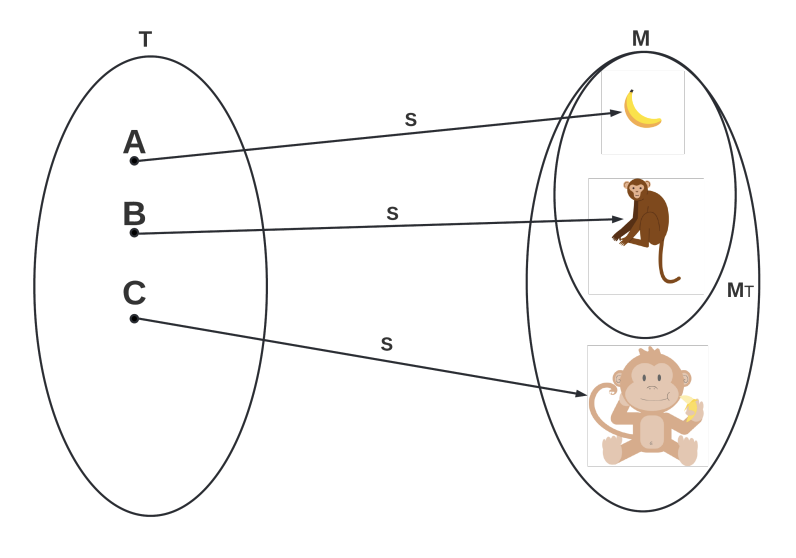
\includegraphics[width=\textwidth]{imgs/ex6.5.png}
    \end{minipage}
\end{myexercise}


\begin{myexercise} \newline
    Considera le frasi e la modellazione della teoria. Determina se è completa, corretta, completa e corretta, incompleta o errata.

    \begin{minipage}{0.6\textwidth}
        \begin{itemize}
            \item A = "There is a banana"
            \item A = "There is a monkey"
            \item C = "There is a tree"
            \item D = "The monkey is eating a banana"        
        \end{itemize}    
    \end{minipage}%
    \begin{minipage}{0.4\textwidth}
        \centering
        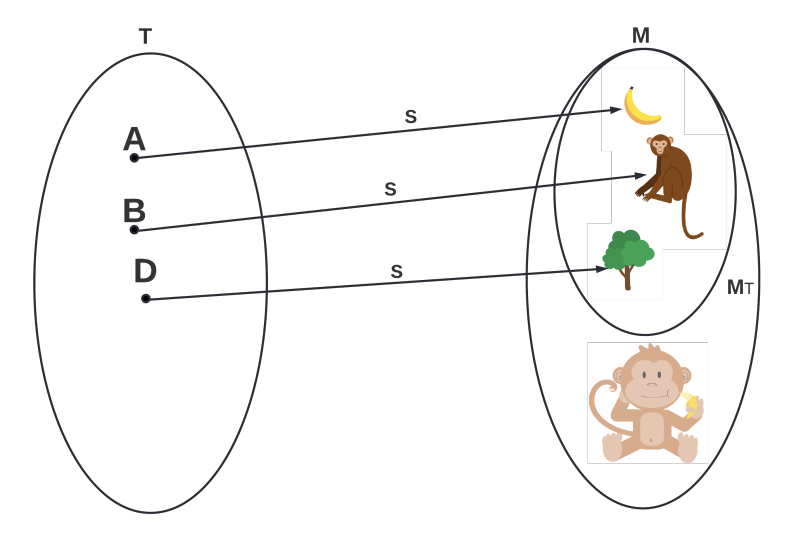
\includegraphics[width=\textwidth]{imgs/ex6.6.png}
    \end{minipage}
\end{myexercise}


\chapter{Grafi di conoscenza - rappresentare il mondo come un grafo}

Rappresentiamo i modelli del mondo \( \hat{W} = \langle L_A, D, I_A \rangle \) come modelli di knowledge graph formalmente rappresentati come \( \mathcal{\hat{KG}} = \langle L_{KG}, D, I_{KG} \rangle \), ossia come tipi speciali di grafi con etichette in cui ogni tripla \( \langle \text{nodo, arco, nodo} \rangle \) \( \in L_{KG} \) è un'affermazione \( a \) \( \in L_{KG} \) che descrive un fatto \( f \) \( \in D \), con \( f = I_{KG}(a) \). Chiamiamo le teorie in \( L_{KG} \) knowledge graphs e utilizziamo la notazione \( KG \subseteq L_{KG} \). Analogamente ai modelli del mondo, distinguiamo tra i modelli \( \mathcal{\hat{KG}} \) che rappresentano dati, conoscenza o informazioni miste.

\begin{mydefinition}[(Entità, etipo e mixed \( \mathcal{\hat{KG}} \)):]

    \begin{itemize}
        \item Un \( \mathcal{\hat{KG}} \) che è un modello di mondo dei dati è chiamato \textit{entity graph model} ($ \mathcal{\hat{EG}} $).
        \item Un \( \mathcal{\hat{KG}} \) che è un modello di mondo della conoscenza è chiamato \textit{etype graph model} ($ \mathcal{\hat{ETG}} $).
        \item Un \( \mathcal{\hat{KG}} \) che è un modello di mondo misto è chiamato \textit{etype entity graph model} ($ \mathcal{ \hat{EEG}} $).
    \end{itemize}

    Questa terminologia si estende in modo ovvio a tutti i componenti di \( \mathcal{\hat{KG}} \), così come a tutti i \( \mathcal{\hat{KG}} \) e modelli correlati definiti all'interno di un \( \mathcal{\hat{KG}} \).

\end{mydefinition}

\section{Dominio}

Sia $\verb|KG = D|^i = \langle E, \{C\} \{R\} \rangle $ lo stencil di un dominio $KG$. Definiamo i suoi componenti.

\begin{mydefinition}[(L'Universo di Interpretazione E di un KG)]
    L'Universo di Interpretazione E di un KG è definito come
    \begin{equation}
        \verb|E = ET| \cup \verb|DT|
    \end{equation}

    con $\verb|ET| \cap \verb|DT| = \emptyset$, dove $\verb|ET = |\{\verb|E|_\textnormal{T}\}$ con $\verb|E|_\textnormal{T} = \{\verb|e|\}$, e $\verb|DT| = \{\verb|D|_\textnormal{T}\}$ con $\verb|D|_\textnormal{T} = \{\verb|v|\}$ \\
    $\verb|E|_\textnormal{T}$ è un \textbf{entity type} (\textbf{etype}) è $\verb|D|_\textnormal{T}$ è un \textbf{datatype} (\textbf{dtype}). Gli elementi degli etype sono chiamati entità, quelli dei dtipi sono chiamati valori (dati).
\end{mydefinition}

\begin{myobservation}[(Etype, dtype)]
    In un KG, \(E\) è strutturato in un insieme di sotto-universi, cioè etipi e dtipi. In astratto, ciascun sotto-universo è simile a una classe \(C \in \{C\}\), ovvero un sottoinsieme di \(E\). La differenza fondamentale è che etipi e dtipi sono tipi che, come nei linguaggi di programmazione, vengono definiti quando si definisce LKG e sono quindi indipendenti dall'applicazione. In quanto tali, questi tipi sono dotati di determinate proprietà e operatori di tipo incorporati, in particolare: un insieme di costruttori che consentono di creare gli elementi di un tipo, un riconoscitore in grado di determinare se un certo elemento appartiene a un certo tipo e una relazione di equivalenza che consente di decidere se due elementi di quel tipo sono uguali.
\end{myobservation}

\begin{myexample}[(Etype)]
    Un esempio di etipo è: \verb|Location|, in cui intuitivamente una \verb|location| è un etipo che contiene spazialmente altre entità. Le locations di solito non cambiano la loro posizione rispetto ai loro sistemi di riferimento delle coordinate. Le loro coordinate spaziali sono quindi un importante indicatore per decidere se due locations (ossia due entità che appartengono all'etipo \verb|Location|) sono effettivamente la stessa location. Ci sono molti etipi che sono casi speciali (sottoetipi) di Location, ad esempio: \verb|Mountain|, \verb|City|, \verb|Street|, \verb|Home| e molti altri. Altri etipi importanti sono: Entity, il più generale etipo, quello che contiene tutti gli elementi in ET (la sua proprietà più evidente è che ha un nome, implementando così il requisito che tutte le entità devono avere un nome); \verb|Event|, le cui proprietà più caratterizzanti sono i tempi di inizio e di fine, \verb|Person|, le cui proprietà più caratterizzanti sono il nome, la data di nascita e i genitori; e molti altri.
\end{myexample}

\begin{myobservation}[(Dtype)]
    
\end{myobservation}
I dtipi hanno le stesse proprietà degli etipi, ma ne aggiungono altre due:
\begin{itemize}
    \item l'insieme dei loro membri, cioè dei loro valori, è predefinito 
    \item i nomi dei valori sono gli stessi dei valori stessi (cioè i valori dei dati si denotano da soli, quindi, ad esempio, il numero (propriamente chiamato numero) 3,14 è il nome del numero 3,14).
\end{itemize}

\begin{myexample}[(Dtype)]
    La seguente è una lista non esaustiva di tipi di dati:
    \begin{verbatim}
        Dtype, Float, Integer, Boolean, String, SpaceTime, Identifier
    \end{verbatim}
    dove \verb|Float, Integer, Boolean, String| definiscono rispettivamente lo spazio dei numeri reali, degli interi, dei valori booleani e delle stringhe. SpaceTime è l'insieme di valori utilizzati per descrivere spazio e tempo. Pertanto, i sotto-tipi di SpaceTime includono GeoCoordinate, Distance, XYCoordinate ma anche Date, Time, DateTime e così via. Dtype è l'insieme di tutti i valori dei dati.
\end{myexample}

\begin{myobservation}[(Set di classi {C} di un KG)]
    Le classi di KG sono classi di modelli del mondo "così come sono", vedere la Definizione 6.1.
\end{myobservation}

\begin{mydefinition}[(Le relazioni binarie tra oggetti e dati {R} di un KG.)]
    L'insieme di relazioni \{R\} = \{OR\} $\cup$ \{DR\} è un insieme di relazioni binarie di un KG tale che
    \begin{equation}
        \verb|R| \subseteq \verb|E|_{\textnormal{T}_s} \times \{\verb|E|_{\textnormal{T}_T} \cup \verb|D|_{\textnormal{T}_t}\}
    \end{equation}
    con $\verb|ET|_s$, $\verb|ET|_t$ $\in$ $\verb|ET|$ e $\verb|DT|_t$ $\in$ $\verb|DT|$. Se R è definito come:
    \begin{equation}
        \verb|R| \subseteq \verb|E|_{E_t} \times \verb|E|_{E_t} 
    \end{equation}

    allora diciamo che R è una relazione oggetto binaria $\verb|OR| \in \{\verb|OR|\}$. Se R è definito come:

    \begin{equation}
        \verb|R| \subseteq \verb|E|_{tT} \times \verb|D|_{T_t}
    \end{equation}

    allora diciamo che R è una relazione dati binaria $\verb|DR| \in \{\verb|DR|\}$.
\end{mydefinition}

\begin{myobservation}[(Arità di una relazione R)]
    In un KG ci sono solo relazioni binarie, ciò consente l'uso di grafi con archi di ingresso e uscita singoli. La rappresentazione di un modello del mondo con archi più complessi richiede la sua riformulazione per consentire solo archi uno-a-uno.
\end{myobservation}

\begin{myobservation}[(Argomenti di una relazione R)]
    Diversamente dalla Definizione 6.1, le relazioni prendono come argomenti etipi e dtipi. Vedere l'Osservazione 7.1 per una spiegazione. Successivamente vedremo come reintrodurre relazioni che prendono come argomenti concetti definiti dall'utente.
\end{myobservation}

\begin{myobservation}[(Relazione tra oggetti)]
    Le relazioni tra oggetti sono relazioni tra entità, rappresentando quindi come le entità interagiscono. Pertanto, ad esempio, alcuni esempi sono:

    $\verb|Near(Person, Tree), HasFather(Person, Person), TalksTo(Person, Dog)|$.
    Si noti che $\verb|Person, Tree, Person, Dog|$ sono etipi, piuttosto che concetti.
\end{myobservation}

\begin{myobservation}[(Relazione dati)]
    Le relazioni dati rappresentano le proprietà delle entità come tali, indipendentemente dalle loro interazioni con altre entità. Ad esempio, alcuni esempi sono: 

    $\verb|Height(Person, Float), HasName(Person, String), HasId(Entity, Identifier)|$.
    Si noti che $\verb|Float, String, Identifier|$ sono dtipi, piuttosto che concetti, come era il caso nella Sezione 5.
\end{myobservation}

\begin{myobservation}[(Relazione, cardinalità)]
    La cardinalità di una relazione può essere: 1-a-1, 1-a-$n$, $m$-a-$n$ (dove uno tra $m$ o $n$ può anche essere 0, il che significa che possono esistere entità che non appartengono a nessuna relazione).
    \begin{figure}[ht]
        \centering
        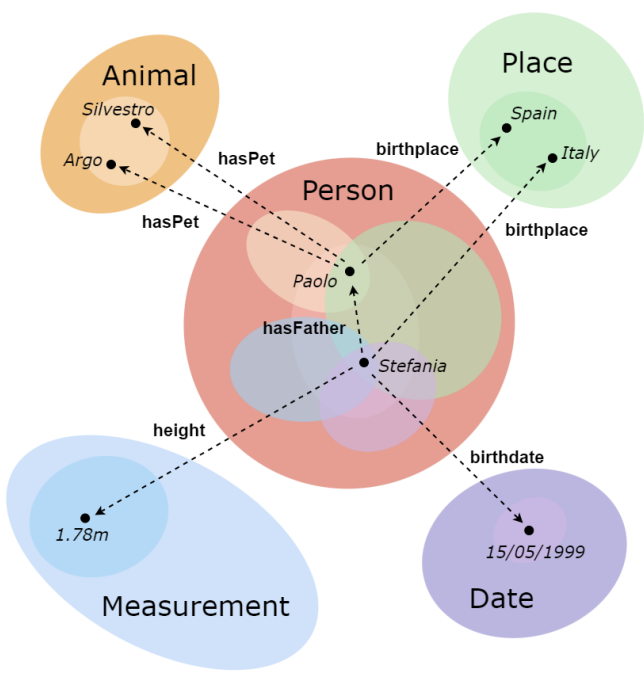
\includegraphics[width=0.7\linewidth]{imgs/img7.1.png}
        \caption{diagramma di Venn di un EG}
    \end{figure}
\end{myobservation}

\begin{myexample}[(Dominio in un \(\hat{\mathcal{EG}}\), Diagramma di Venn)]
    Rappresentiamo i domini degli EG come nella Figura 7.1. Le relazioni sono rappresentate come collegamenti tra entità dell'etipo appropriato e entità o valori dell'etipo o del dtipo appropriato, rispettivamente.
\end{myexample}

\begin{myexample}[(Dominio in \(\hat{\mathcal{ETG}}\), Diagramma di Venn)]
    Rappresentiamo i domini degli ETG come nella Figura 7.1. Le relazioni sono rappresentate come collegamenti tra etipi ed etipi/dtipi.
\end{myexample}

\clearpage
\begin{figure}[ht]
    \centering
    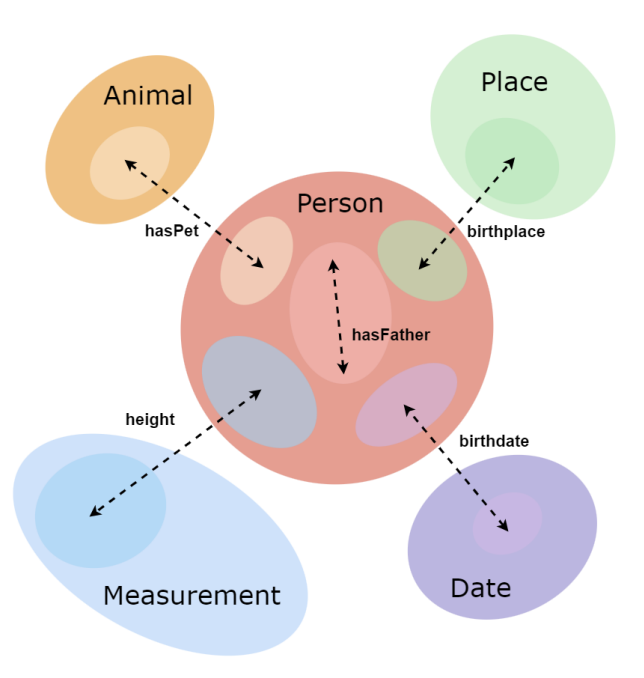
\includegraphics[width=0.7\linewidth]{imgs/img7.2.png}
    \caption{diagramma di Venn di un ETG}
\end{figure}

\section{Linguaggio assertivo}

Sia $\mathcal{L}^i_{\mathcal{KG}} = \mathcal{L}^i_{\mathcal{A}} = \langle \mathcal{E}, \{\mathcal{C}\} \{\mathcal{P}\} \rangle$ lo stencil del $\hat{\mathcal{KG}}$ linguaggio $L^i_{\mathcal{KG}}$. La definizione di $L^i_{\mathcal{KG}}$ segue direttamente dalla definizione di $\verb|D|^i$ nella Sezione 7.1.

\begin{mydefinition}[(Concetto)]
    Abbiamo
    \begin{equation}
        \{\mathcal{C}\} = \mathcal{ET} \cup \mathcal{DT}
    \end{equation}

    dove $\mathcal{ET} = \{\mathcal{E}_\mathcal{T}\}$ e $\mathcal{DT} = \mathcal{D}_\mathcal{T}$ sono rispettivamente (nomi dei) \textbf{etipi} e \textbf{dtipi} in $\hat{\mathcal{KG}}$
\end{mydefinition}

\begin{mydefinition}[(Proprietà degli oggetti e dei dati)]
    \begin{equation}
        \{\mathcal{P}\} = \{\mathcal{OP}\} \cup \{\mathcal{DP}\}
    \end{equation}
    dove $\{\mathcal{OP}\}$ e $\{\mathcal{DP}\}$ sono definiti come segue:
    
    \begin{equation}
        \begin{aligned}
            \{\mathcal{OP}\} \subseteq \{\mathcal{E_T}\} \times \{\mathcal{E_T}\} \\
            \{\mathcal{OP}\} \subseteq \{\mathcal{E_T}\} \times \{\mathcal{E_T}\}
        \end{aligned}
    \end{equation}

    Gli elementi di $\{\mathcal{OP}\}$ sono chiamati proprietà degli oggetti, quelli di $\{\mathcal{DP}\}$ proprietà dei dati.
\end{mydefinition}

\begin{myexample}[(\(\mathcal{EG}\))]
    L'$\mathcal{EG}$ di questo esempio rappresenta il dominio descritto nell'Esempio 7.3. La chiave dell'osservazione sta nel fatto che il numero di nodi corrisponde al numero di entità e valori, mentre il numero di archi corrisponde ai valori di proprietà istanziate. Si noti come i vincoli di cardinalità $n$-a-$m$ consentano agli archi etichettati con la stessa proprietà di uscire dallo stesso nodo di etipi. Si noti anche come i nodi di dati siano e possano essere solo nodi foglia.
\end{myexample}

\begin{figure}[ht]
    \centering
    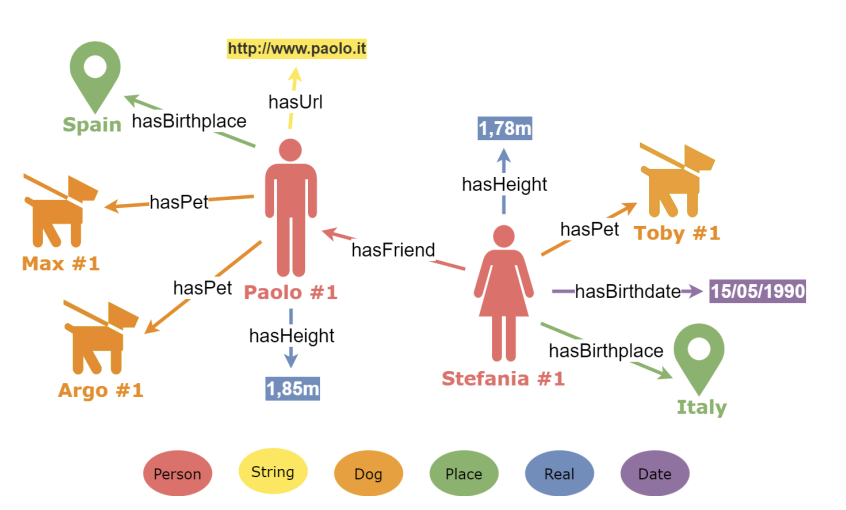
\includegraphics[width=0.7\linewidth]{imgs/img7.3.png}
    \caption{Esempio di un EG che rappresenta informazioni riguardo agli esseri umani.}
\end{figure}


\begin{myexample}[\(\mathcal{ETG}\)]
    L'$\mathcal{ETG}$ di questo esempio rappresenta il dominio descritto nell'Esempio 7.4. C'è un nodo per etipo e tipo di dati. L'$\mathcal{ETG}$ codifica alcune meta-informazioni, ad esempio i vincoli di cardinalità, che possono guidare e controllare la creazione dell'$\mathcal{EG}$ a partire da un $\mathcal{ETG}$. In modo simile agli $\mathcal{EG}$, i nodi dei dtipi sono nodi foglia.
\end{myexample}

\clearpage
\begin{figure}[ht]
    \centering
    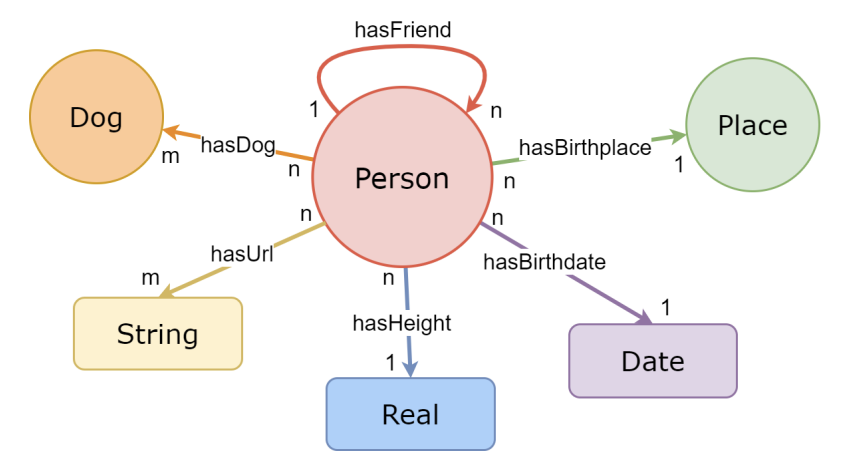
\includegraphics[width=0.7\linewidth]{imgs/img7.4.png}
    \caption{Esempio di un ETG che rappresenta informazioni riguardo agli esseri umani.}
\end{figure}


\begin{myobservation}[(\(\hat{\mathcal{EG}} , \hat{\mathcal{ETG}}, \hat{\mathcal{EEG}} \))]
    Nelle affermazioni di $\hat{\mathcal{KG}}$, le triple sono < nodo, arco, nodo > $\in \mathcal{L}_A$. Nei nodi di $\hat{\mathcal{KG}}$, i nodi $\hat{\mathcal{EG}}$ rappresentano o entità con il loro etipo o valori con il loro dtype. Nei nodi di $\hat{\mathcal{ETG}}$, i nodi rappresentano etipi. Nei nodi di $\hat{\mathcal{EEG}}$, ci sono entrambi i tipi di nodi. Gli archi sono etichettati con nomi di proprietà e rappresentano relazioni. Gli archi da etipi/entità a etipi/entità rappresentano relazioni tra oggetti. Gli archi da etipi/entità a dtipi/valori rappresentano relazioni tra dati.
\end{myobservation}

\section{Funzione di interpretazione}
La funzione di interpretazione di un $\hat{\mathcal{KG}}$ è una mappatura diretta dal linguaggio assertivo $\mathcal{L}^i_{\mathcal{KG}}$ al dominio di interpretazione di destinazione $\verb|D|$. Come si può vedere dagli esempi nella Sezione 7.1 e nella Sezione 7.2, esiste una mappatura quasi diretta tra il linguaggio e il dominio di interpretazione. In pratica, ciò significa che una volta che è stata chiarita la denotazione degli elementi del singolo linguaggio di $\mathcal{L}_{\mathcal{KG}}$ e ci si è assicurati che la funzione di interpretazione soddisfi tutti i requisiti (vedi Sezione 6.4), il significato previsto di un $\mathcal{KG}$ può essere letto direttamente dal $\mathcal{KG}$ stesso.

\section{Grafo di conoscenza}
I modelli di grafo della conoscenza del mondo $\hat{\mathcal{KG}} = \langle \mathcal{L}^i_{\mathcal{KG}}, \verb|D|^i, \mathcal{I}^i_{KG}\rangle $ sono una rappresentazione universale, intuitiva, autoesplicativa ed efficiente dal punto di vista computazionale del mondo.
Una volta fornito un $\hat{\mathcal{KG}}$, è sufficiente per costruire il proprio $\mathcal{KG}$  preferito e tutte le operazioni descritte nella Sezione 6.5 sono disponibili.

\begin{myobservation}[(Tipi di grafi di conoscenza)]
    Come discusso anche nell'Osservazione 6.3, i modelli del mondo e i grafi di conoscenza introdotti finora hanno un'espressività minima. In pratica, i grafi di conoscenza sono spesso arricchiti con ulteriori costruttori che consentono la descrizione di fatti più complessi. Questa è un'operazione del tutto valida con l'avvertenza che è necessario fare attenzione nella selezione del giusto compromesso tra complessità, intuitività e complessità computazionale della rappresentazione selezionata.
\end{myobservation}

\begin{myobservation}[(Dai grafi di conoscenza alla logica)]
    I $\mathcal{KG}$ consentono una facile incorporazione nella logica più appropriata con l'obiettivo di consentire il ragionamento su di essi. Questo sarà l'argomento delle sezioni successive.
\end{myobservation}

\section{Esercizi}

\begin{myexercise}[(Crea un diagramma di insiemi)]
    Considera questa mappa della metropolitana di Milano:
    \begin{figure}[ht]
        \centering
        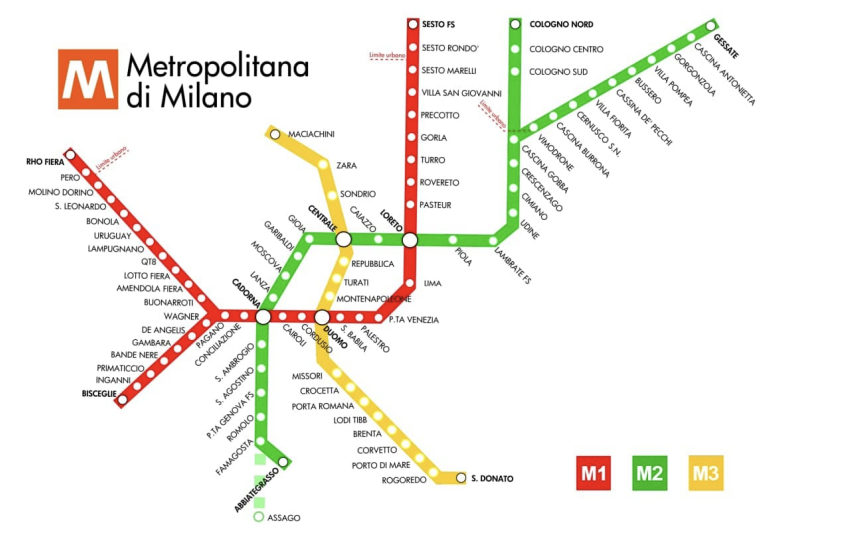
\includegraphics[width=0.7\linewidth]{imgs/img7.5.png}
        \caption{Mappa della metropolitana di Milano}
    \end{figure}

    Cosa deve essere fatto:
    \begin{itemize}
        \item Estrarre insiemi rilevanti di oggetti: Linee, Stazioni, Incroci, Terminali, Numero di stazioni, Colori, ...
        \item Istanziare elementi del dominio: Linea rossa, Cadorna, RHO fiera, Milano, Giallo
        \item Estrarre relazioni rilevanti: haColore, appartieneA, faParteDi, vicinoA, ...
    \end{itemize}
\end{myexercise}

\chapter{Rappresentazione estensionale della logica}

\end{document}